% =====================================================================
%  preamble.tex : the one preamble of the paper style (tikz-figures)
%
%  Two ways to use it. While working, a figure file starts with
%      \def\figpreambleonly{}
%      % =====================================================================
%  preamble.tex : the one preamble of the paper style (tikz-figures)
%
%  Two ways to use it. While working, a figure file starts with
%      \def\figpreambleonly{}
%      % =====================================================================
%  preamble.tex : the one preamble of the paper style (tikz-figures)
%
%  Two ways to use it. While working, a figure file starts with
%      \def\figpreambleonly{}
%      % =====================================================================
%  preamble.tex : the one preamble of the paper style (tikz-figures)
%
%  Two ways to use it. While working, a figure file starts with
%      \def\figpreambleonly{}
%      \input{preamble.tex}
%  and then has its own document environment with one tikzpicture. To
%  deliver, inline it (scripts/render_figure.py --inline OUT.tex copies
%  everything above the line "%%%% FIGURE BODY" into the file), so the
%  delivered figure needs no other file. The body below that line is a
%  smoke test that draws every element once; it makes this file compile
%  alone and is skipped when \figpreambleonly is defined.
%
%  Type: the TeX default, Computer Modern text and default math. fix-cm
%  allows arbitrary sizes. There is no font encoding package, no sans
%  text or math package, no mathastext and no lmodern here, and no sans
%  option: the author decided the font once ("make both figures default
%  tikz/tex font").
%
%  Colors are named by ROLE and defined once. A paper that needs another
%  value redefines that one name after this block (\definecolor{...});
%  that is the only knob. There is no theme switch.
%
%  Sizes are DESIGN sizes. The figures of this style are drawn large and
%  printed small (a card figure 850 bp wide printed at 388 bp, scale
%  0.457). Check the printed sizes with scripts/print_scale.py on the
%  compiled PDF; nothing may print under the 5 pt floor.
%
%  Units: generated figures and block cards use x=1bp, y=1bp (PDF big
%  points; a TeX point is 0.375 percent smaller, enough to slide a patch
%  off the artwork). Overviews and compositions use cm, as the source
%  figures did. Every macro below states its unit.
%
%  The \newcommand\fig... number lines are read by assets/figkit.py, so a
%  hand-written figure and a generated one share every size. Keep each
%  on one line in the form \newcommand\figName{number}.
%
%  Compile: pdflatex -interaction=nonstopmode -halt-on-error fig.tex
%  Needs: standalone, tikz, pgfplots (in a full TeX Live; BasicTeX needs
%  standalone and pgfplots added).
% =====================================================================
\documentclass[border=4pt]{standalone}
\usepackage{fix-cm}
\usepackage{amsmath,amssymb}
\usepackage{graphicx}
\usepackage{tikz}
\usetikzlibrary{arrows.meta,decorations.pathreplacing,calc}
\usepackage{pgfplots}
\pgfplotsset{compat=1.18}
\usepgfplotslibrary{fillbetween}

% ---------------------------------------------------------------------
%  NUMBERS (bp unless stated). Measured from the author's latest paper
%  figures with PyMuPDF; references/style.md gives the source of each.
% ---------------------------------------------------------------------
% block cards
\newcommand\figBoxW{92}        % every plain box (LayerNorm, FFN, ...)
\newcommand\figBoxH{28}
\newcommand\figOpW{136}        % the one operation box of a block
\newcommand\figOpH{40}
\newcommand\figBoxR{1.6}       % box corner radius
\newcommand\figCardR{3.0}      % card corner radius
\newcommand\figHeadL{3.9}      % flat-backed arrowhead, length
\newcommand\figHeadW{3.0}      % and width
\newcommand\figJoinR{5.6}      % join circle radius
\newcommand\figDotR{1.0}       % junction dot radius
\newcommand\figChip{4.4}       % one chip cell
\newcommand\figChipGap{1.2}    % gap between cells of a token
\newcommand\figChipCols{4}     % cells in a token row
\newcommand\figStackRows{4}    % rows in a K-deep stack
\newcommand\figStackOff{2.8}   % each row offset up and right by this
\newcommand\figMini{6.0}       % mini icon cell
\newcommand\figMiniGap{1.5}    % mini icon gap
\newcommand\figNameInset{12}   % card name starts this far right of the card edge
\newcommand\figNameDrop{0.32}  % card name baseline below the border, in units of its size
% line widths (TeX pt; 0.4 pt prints as the measured 0.3985 bp)
\newcommand\figLwCard{0.40}
\newcommand\figLwChip{0.40}
\newcommand\figLwWire{0.45}
\newcommand\figLwRes{0.40}
\newcommand\figLwMini{0.35}
\newcommand\figLwFlow{0.70}    % overview wires
\newcommand\figLwRail{0.60}    % feedback rails of a hierarchy
% type at design scale (TeX pt)
\newcommand\figPtName{14.0}    % card name on the border
\newcommand\figPtCap{13.6}     % stream captions, output caption, legend line
\newcommand\figPtBox{13.2}     % text inside boxes
\newcommand\figPtNote{13.0}    % gloss, wire labels, symbols beside glyphs
\newcommand\figPtLabel{13.0}   % overview labels
\newcommand\figPtSlab{10.0}    % two-line labels inside encoder slabs
\newcommand\figPtGloss{11.0}   % overview gloss
\newcommand\figPtTitle{16.0}   % composition panel title
\newcommand\figPtTile{13.5}    % label over a data tile
\newcommand\figPtCount{12.5}   % count or caption under a tile
\newcommand\figPtLetter{20.0}  % a bare panel letter (bold)

% font switches, one per role
\newcommand\fName{\fontsize{\figPtName}{16.8}\selectfont}
\newcommand\fCap{\fontsize{\figPtCap}{16.3}\selectfont}
\newcommand\fBox{\fontsize{\figPtBox}{15.8}\selectfont}
\newcommand\fNote{\fontsize{\figPtNote}{15.6}\selectfont}
\newcommand\fLabel{\fontsize{\figPtLabel}{15.6}\selectfont}
\newcommand\fSlab{\fontsize{\figPtSlab}{12}\selectfont}
\newcommand\fGloss{\fontsize{\figPtGloss}{13.2}\selectfont}
\newcommand\fTitle{\fontsize{\figPtTitle}{19.2}\selectfont}
\newcommand\fTile{\fontsize{\figPtTile}{16.2}\selectfont}
\newcommand\fCount{\fontsize{\figPtCount}{15}\selectfont}
\newcommand\fLetter{\fontsize{\figPtLetter}{24}\selectfont\bfseries}

% ---------------------------------------------------------------------
%  COLORS BY ROLE (hex measured from the paper figures)
% ---------------------------------------------------------------------
\colorlet{ink}{black}                       % wires and text
\colorlet{glossink}{black!70}               % secondary text: gloss, wire labels, symbols
\definecolor{boxline}{HTML}{333333}         % outline of every box
\definecolor{chipline}{HTML}{404040}        % outline of token chips
\definecolor{miniline}{HTML}{666666}        % outline of the what-it-does icon
\definecolor{cardline}{HTML}{B2B2B2}        % card frame
% token fills: a chip color names a KIND of token in every panel
\definecolor{tokblue}{HTML}{93B4D8}
\definecolor{tokorange}{HTML}{F0B060}
\definecolor{tokpurple}{HTML}{B9A3DC}
\definecolor{tokgreen}{HTML}{8FBFA0}
\definecolor{tokyellow}{HTML}{F5D36B}       % the leaf chips; also the selected path
% the one filled box of a block; every other box is white
\definecolor{oppeach}{HTML}{FBE0C2}         % cross-attention, pooling
\definecolor{opmint}{HTML}{D8E9DF}          % self-attention, neighborhood
\definecolor{opgray}{HTML}{E8E8E8}          % graph layer
% overview fills
\definecolor{slabgray}{HTML}{E8E8EC}        % encoder slab with a domed top
\definecolor{wheat}{HTML}{F5E2B0}           % predictor with a D-shaped cap
\definecolor{panelgray}{HTML}{F4F4F5}       % a faded module, shown but outside the claim
% the single loss box
\definecolor{lossline}{HTML}{D93025}
\definecolor{lossfill}{HTML}{FBE9E7}
% points, their density washes, graph edges
\definecolor{ptblue}{HTML}{5C8CC4}
\definecolor{ptochre}{HTML}{C98F3D}
\definecolor{ptpurple}{HTML}{9475B5}
\definecolor{washblue}{HTML}{A9C3E2}
\definecolor{washochre}{HTML}{E6D4AE}
\definecolor{washpurple}{HTML}{CDBBDF}
\colorlet{edgeline}{black!40}
% frames, masks, connectors, rules
\colorlet{cropline}{black!45}
\colorlet{queryline}{black!55}
\colorlet{zoomboxline}{black!75}
\colorlet{zoomline}{black!30}
\colorlet{maskline}{black!40}
\colorlet{maskfill}{black!5}
\colorlet{maskedpt}{black!13}
\colorlet{tileline}{black!28}
\colorlet{ruleline}{black!22}
% hierarchy
\definecolor{tilepale}{HTML}{FCEFC4}        % context tiles of the pyramid
\colorlet{tilestrong}{tokyellow}            % the selected path: tiles and tree nodes
\colorlet{treeedge}{black!55}
% sphere glyph
\colorlet{graticule}{black!22}
% sequential ramp of the package (data-figures RANK5): light to dark
\definecolor{ramp1}{HTML}{F1F6FF}
\definecolor{ramp2}{HTML}{C7DCFF}
\definecolor{ramp3}{HTML}{8FB9FF}
\definecolor{ramp4}{HTML}{4D97FF}
\definecolor{ramp5}{HTML}{003FBD}
% data plots: the package's color roles for compared items (data-figures style tokens)
\definecolor{hero}{HTML}{0072B2}            % the method the paper is about
\definecolor{rival}{HTML}{E69F00}           % the strongest comparator
\definecolor{othergray}{HTML}{A8A8AD}       % every other comparator
\definecolor{basegray}{HTML}{6E6E73}        % an untrained or trivial baseline
\definecolor{bandgray}{HTML}{EFEFF1}        % seed-to-seed noise band
\definecolor{guidegray}{HTML}{D1D1D6}       % guide lines and the grid of a heat matrix

% ---------------------------------------------------------------------
%  STYLES
% ---------------------------------------------------------------------
\tikzset{
  paper/.style={line cap=round, line join=round},
  every node/.append style={text=ink},
  % text
  gloss/.style={text=glossink},
  capt/.style={font=\fCap},
  note/.style={font=\fNote, text=glossink},
  lbl/.style={font=\fLabel, align=center},
  glossnote/.style={font=\fGloss, text=glossink, align=center},
  % boxes (bp): one size for every plain box, one for the operation box
  box/.style={draw=boxline, fill=white, line width=\figLwWire pt,
    rounded corners=\figBoxR bp, minimum width=\figBoxW bp, minimum height=\figBoxH bp,
    inner sep=0pt, outer sep=0pt, align=center, font=\fBox},
  opbox/.style={box, fill=#1, minimum width=\figOpW bp, minimum height=\figOpH bp},
  opbox/.default=oppeach,
  % wires (bp family): flat-backed head, stops 1 bp short of a box
  wire/.style={draw=ink, line width=\figLwWire pt,
    -{Triangle[length=\figHeadL bp, width=\figHeadW bp]}},
  wirebare/.style={draw=ink, line width=\figLwWire pt},
  resid/.style={draw=ink, line width=\figLwRes pt,
    -{Triangle[length=\figHeadL bp, width=\figHeadW bp]}},
  residbare/.style={draw=ink, line width=\figLwRes pt},
  chip/.style={draw=chipline, line width=\figLwChip pt},
  mini/.style={draw=miniline, line width=\figLwMini pt},
  bracegloss/.style={draw=glossink, line width=\figLwMini pt, decorate,
    decoration={brace, amplitude=3.2bp, raise=#1}},
  bracegloss/.default=1.4bp,
  % card frame and its name on the border
  card/.style={draw=cardline, line width=\figLwCard pt, rounded corners=\figCardR bp},
  cardname/.style={anchor=base west, fill=white, inner xsep=3bp, inner ysep=3bp,
    outer sep=0pt, font=\fName},
  % overview family (cm): wires, EMA, continuation
  flow/.style={draw=ink, line width=\figLwFlow pt, -{Stealth}},
  flowbare/.style={draw=ink, line width=\figLwFlow pt},
  ema/.style={flow, dashed},
  % hierarchy rails (bp family): Stealth heads as in the hierarchy panel
  rail/.style={draw=ink, line width=\figLwRail pt,
    -{Stealth[length=\figHeadL bp, width=2.9bp]}},
  railbare/.style={draw=ink, line width=\figLwRail pt},
  railcont/.style={rail, dash pattern=on 2.989bp off 2.989bp},
  railcontbare/.style={railbare, dash pattern=on 2.989bp off 2.989bp},
  % overview shapes (outer sep 0: an anchor such as (q.east) lies ON the frame line, so a wire drawn from it
  % starts on the frame and not half a line width outside it)
  qbox/.style={draw=queryline, line width=0.6pt, fill=white, rounded corners=3pt,
    inner xsep=5pt, inner ysep=4pt, outer sep=0pt, align=center, font=\fLabel},
  loss/.style={draw=lossline, line width=0.9pt, fill=lossfill, rounded corners=3pt,
    minimum width=0.90cm, minimum height=0.84cm, inner sep=0pt, outer sep=0pt, font=\fLabel},
  % crops, masks, zoom
  crop/.style={draw=cropline, line width=0.6pt, rounded corners=2pt, fill=white},
  maskbox/.style={draw=maskline, line width=0.6pt, dash pattern=on 1.4pt off 1.2pt,
    fill=maskfill},
  zoombox/.style={draw=zoomboxline, line width=0.55pt},
  zoomlink/.style={draw=zoomline, line width=0.45pt, dash pattern=on 2pt off 1.8pt},
  graphedge/.style={draw=edgeline, line width=0.34pt},
  % composition
  tileframe/.style={draw=tileline, line width=0.4pt},
  panelrule/.style={draw=ruleline, line width=0.4pt},
  paneltitle/.style={anchor=south west, inner sep=2pt, font=\fTitle, align=left},
  tilelabel/.style={font=\fTile, align=center},
  tilecount/.style={font=\fCount, align=center},
  % hierarchy: tree and pyramid
  treenode/.style={circle, draw=ink, line width=0.5pt, fill=white,
    minimum size=11.34bp, inner sep=0pt, outer sep=0pt},
  treeedge/.style={draw=treeedge, line width=0.5pt},
  treepath/.style={draw=ink, line width=1.1pt},
  isotile/.style={draw=ink, line width=0.35pt},
}

% ---------------------------------------------------------------------
%  MACROS (coordinates are any TikZ coordinate; offsets carry their unit)
% ---------------------------------------------------------------------
% a token: a row of #3 chip cells centered on #1, fill #2
\newcommand\tokrow[3]{%
  \pgfmathsetmacro\figRowW{#3*\figChip+(#3-1)*\figChipGap}%
  \pgfmathsetmacro\figHalfC{\figChip/2}%
  \foreach \kk in {1,...,#3}{%
    \pgfmathsetmacro\figCx{-\figRowW/2+(\kk-1)*(\figChip+\figChipGap)}%
    \draw[chip, fill=#2] ($(#1)+(\figCx bp,-\figHalfC bp)$) rectangle ++(\figChip bp,\figChip bp);
  }}
% a set of K tokens: [rows] rows of \figChipCols cells stacked behind one
% another, each row offset up and right; #1 is the FRONT row's center
\newcommand\tokstack[3][\figStackRows]{%
  \pgfmathtruncatemacro\figRm{#1-1}%
  \foreach \ii in {\figRm,...,0}{%
    \pgfmathsetmacro\figOff{\ii*\figStackOff}%
    \tokrow{$(#2)+(\figOff bp,\figOff bp)$}{#3}{\figChipCols}%
  }}
% the stack's width, bracketed over its BACK row (label #3, e.g. $d$)
\newcommand\tokwidthbrace[3][\figStackRows]{%
  \pgfmathsetmacro\figRowW{\figChipCols*\figChip+(\figChipCols-1)*\figChipGap}%
  \pgfmathsetmacro\figBx{(#1-1)*\figStackOff}%
  \pgfmathsetmacro\figTop{\figChip/2+(#1-1)*\figStackOff+1.5}%
  \draw[bracegloss] ($(#2)+(\figBx bp-\figRowW bp/2,\figTop bp)$)
      -- ($(#2)+(\figBx bp+\figRowW bp/2,\figTop bp)$);
  \node[note, anchor=base, inner sep=0pt] at ($(#2)+(\figBx bp,\figTop bp+8.5bp)$) {#3};}
% the stack's COUNT, bracketed along its own diagonal, drawn back to front
% so it bulges away from the stack (label #3, e.g. $K$)
\newcommand\tokdepthbrace[3][\figStackRows]{%
  \pgfmathsetmacro\figRowW{\figChipCols*\figChip+(\figChipCols-1)*\figChipGap}%
  \pgfmathsetmacro\figBk{(#1-1)*\figStackOff}%
  \pgfmathsetmacro\figD{2.2*0.7071}%
  \pgfmathsetmacro\figG{7.0*0.7071}%
  \coordinate (fig@back) at ($(#2)+(\figRowW bp/2+\figBk bp+\figD bp,\figChip bp/2+\figBk bp-\figD bp)$);
  \coordinate (fig@front) at ($(#2)+(\figRowW bp/2+\figD bp,\figChip bp/2-\figD bp)$);
  \draw[bracegloss=0.8bp] (fig@back) -- (fig@front);
  \node[note, anchor=base west, inner sep=0pt] at
    ($(fig@back)!0.5!(fig@front)+(\figG bp,-\figG bp-0.34*\figPtNote bp)$) {#3};}
% join circle with a plus: residual and other additions
\newcommand\joincircle[1]{%
  \draw[ink, fill=white, line width=\figLwWire pt] (#1) circle (\figJoinR bp);
  \pgfmathsetmacro\figArm{0.55*\figJoinR}%
  \draw[ink, line width=\figLwChip pt] ($(#1)+(-\figArm bp,0)$) -- ($(#1)+(\figArm bp,0)$);
  \draw[ink, line width=\figLwChip pt] ($(#1)+(0,-\figArm bp)$) -- ($(#1)+(0,\figArm bp)$);}
% junction dot: where a wire branches
\newcommand\junction[1]{\fill[ink] (#1) circle (\figDotR bp);}
% pre-norm residual: tap #1 (dot), run out to the x of #2, come back into
% the side of the join at #3 that faces the margin
\newcommand\residual[3]{%
  \junction{#1}
  \draw[resid] let \p1=(#2), \p2=(#3) in
    (#1) -- (#1 -| #2) -- (#3 -| #2) -- ($(#3)+({sign(\x1-\x2)*\figJoinR*1bp},0)$);}
% a card: frame with the name ON the top border (border masked by the
% name's own box); #1 top-left corner, #2 width and #3 height in bp
\newcommand\card[4]{%
  \draw[card] (#1) rectangle ++(#2 bp,-#3 bp);
  \pgfmathsetmacro\figNd{\figNameDrop*\figPtName}%
  \node[cardname] at ($(#1)+(\figNameInset bp,-\figNd bp)$) {#4};}
% a two-level label: a black name, its gray gloss 15 bp under it
\newcommand\twolevel[3]{%
  \node[capt, anchor=base, inner sep=0pt] at (#1) {#2};
  \node[note, anchor=base, inner sep=0pt] at ($(#1)+(0,-15bp)$) {#3};}
% mini icons, #1 = top-left corner. pool: four children to one parent
\newcommand\minipool[1]{%
  \pgfmathsetmacro\figP{\figMini+\figMiniGap}%
  \foreach \ii in {0,1}{\foreach \jj in {0,1}{%
    \draw[mini, fill=tokblue] ($(#1)+(\ii*\figP bp,-\jj*\figP bp)$) rectangle ++(\figMini bp,-\figMini bp);}}
  \pgfmathsetmacro\figH{2*\figP-\figMiniGap}%
  \fill[ink] ($(#1)+(\figH bp+3bp,-\figH bp/2+2bp)$) -- ++(4bp,-2bp) -- ++(-4bp,-2bp) -- cycle;
  \draw[chip, line width=\figLwMini pt, fill=tokorange] ($(#1)+(\figH bp+10bp,0)$) rectangle ++(\figH bp,-\figH bp);}
% mix: a tile and its neighborhood to that tile
\newcommand\minimix[1]{%
  \pgfmathsetmacro\figP{\figMini+\figMiniGap}%
  \foreach \ii in {0,1,2}{\foreach \jj in {0,1,2}{%
    \pgfmathsetmacro\figCtr{(\ii==1)&&(\jj==1)}%
    \ifdim\figCtr pt>0.5pt\def\figF{tokorange!70!black}\else\def\figF{tokorange}\fi
    \draw[mini, fill=\figF] ($(#1)+(\ii*\figP bp,-\jj*\figP bp)$) rectangle ++(\figMini bp,-\figMini bp);}}
  \pgfmathsetmacro\figH{3*\figP-\figMiniGap}%
  \fill[ink] ($(#1)+(\figH bp+3bp,-\figH bp/2+2bp)$) -- ++(4bp,-2bp) -- ++(-4bp,-2bp) -- cycle;
  \draw[mini, fill=tokblue] ($(#1)+(\figH bp+10bp,-\figP bp)$) rectangle ++(\figMini bp,-\figMini bp);}
% read: tiles coarse to fine to one point
\newcommand\miniread[1]{%
  \pgfmathsetmacro\figP{\figMini+\figMiniGap}%
  \foreach \ii in {0,1,2}{%
    \pgfmathsetmacro\figS{\figMini*(1-0.2*\ii)}%
    \draw[mini, fill=tokblue] ($(#1)+(\ii*\figP bp,-\figMini bp/2+\figS bp/2)$) rectangle ++(\figS bp,-\figS bp);}
  \pgfmathsetmacro\figXa{3*\figP-\figMiniGap+3}%
  \fill[ink] ($(#1)+(\figXa bp,-\figMini bp/2+2bp)$) -- ++(4bp,-2bp) -- ++(-4bp,-2bp) -- cycle;
  \fill[chipline] ($(#1)+(\figXa bp+9bp,-\figMini bp/2)$) circle (2.2bp);}
% the unit sphere glyph of a card: outline, equator, one unit vector's dot
\newcommand\unitsphere[2]{% #1 center, #2 radius in bp
  \draw[mini] (#1) circle (#2 bp);
  \draw[mini] (#1) ellipse ({#2 bp} and {0.36*#2 bp});
  \fill[ink] ($(#1)+(0.44*#2 bp,0.52*#2 bp)$) circle (2.2bp);}
% overview (cm): encoder slab with a domed top; #1 bottom-left, #2 width in cm
\newcommand\slab[3]{%
  \path[fill=slabgray] (#1) -- ++(#2 cm,0) -- ++(0,0.82cm)
     .. controls +(0,0.55cm) and +(0,0.55cm) .. ++(-#2 cm,0) -- cycle;
  \node[font=\fSlab, align=center] at ($(#1)+(#2 cm/2,0.55cm)$) {#3};}
% predictor with a D-shaped cap; #1 bottom-left, #2 straight width, #3 height (cm)
\newcommand\dcap[4]{%
  \path[rounded corners=3pt, fill=wheat] (#1) -- ++(#2 cm,0)
     arc[start angle=-90, end angle=90, radius=#3 cm/2] -- ++(-#2 cm,0) -- cycle;
  \node[lbl] at ($(#1)+(#2 cm/2+#3 cm/8,#3 cm/2)$) {#4};}
% stop-gradient: two short parallel slashes across a vertical wire at #1;
% [90] turns them for a horizontal wire
\newcommand\stopgrad[2][0]{%
  \begin{scope}[rotate around={#1:(#2)}]
    \draw[ink, line width=\figLwFlow pt] ($(#2)+(-0.17cm,-0.17cm)$) -- ++(0.34cm,0.18cm);
    \draw[ink, line width=\figLwFlow pt] ($(#2)+(-0.17cm,-0.01cm)$) -- ++(0.34cm,0.18cm);
  \end{scope}}
% points (cm family): a point, a masked point, a graph node
\newcommand\figpoint[2]{\fill[#2, opacity=0.9] (#1) circle (0.032cm);}
\newcommand\figmasked[1]{\fill[maskedpt] (#1) circle (0.028cm);}
\newcommand\fignode[2]{\fill[#2, opacity=0.9] (#1) circle (0.052cm);}
% hierarchy: an isometric tile, #1 center, #2 half-width (bp), #3 fill
\newcommand\isotile[3]{%
  \draw[isotile, fill=#3] ($(#1)+(-#2 bp,0)$) -- ($(#1)+(0,#2 bp/2)$)
     -- ($(#1)+(#2 bp,0)$) -- ($(#1)+(0,-#2 bp/2)$) -- cycle;}
% composition (cm): a raster tile with its hairline frame; #1 x, #2 y
% (center), #3 width in cm, #4 file
\newcommand\tile[4]{%
  \node[inner sep=0pt] at (#1,#2) {\includegraphics[width=#3cm]{#4}};
  \draw[tileframe] ({#1-#3/2},{#2-#3/2}) rectangle ({#1+#3/2},{#2+#3/2});}
% a panel title: bold letter, parenthesis, two spaces, a short name
\newcommand\paneltitle[3]{\node[paneltitle] at (#1) {\textbf{#2)}\ \ #3};}
% a bare panel letter (bold, one size and one baseline for every letter)
\newcommand\panelletter[2]{\node[anchor=base west, inner sep=0pt, font=\fLetter] at (#1) {#2};}

% ---------------------------------------------------------------------
%  PGFPLOTS: plots are drawn at their PRINTED size, so their type is the
%  package's on-page tiers (7 pt titles, 6 pt labels, 5 pt ticks).
% ---------------------------------------------------------------------
\pgfplotsset{
  paperaxis/.style={
    axis lines=left, axis line style={-, draw=black!93, line width=0.5pt},
    tick align=outside, tick style={draw=black!93, line width=0.4pt},
    major tick length=1.8pt, minor tick length=0pt,
    every tick label/.append style={font=\fontsize{5}{6}\selectfont},
    label style={font=\fontsize{6}{7.2}\selectfont},
    title style={font=\fontsize{7}{8.4}\selectfont, yshift=-2pt},
    every axis plot/.append style={line width=0.8pt},
    legend style={draw=none, fill=none, font=\fontsize{5}{6}\selectfont},
    clip=false, scale only axis,
  },
  colormap={rank5}{color=(ramp1) color=(ramp2) color=(ramp3) color=(ramp4) color=(ramp5)},
}

%%%% FIGURE BODY: the preamble ends above this line; below is the smoke test
\ifdefined\figpreambleonly\expandafter\endinput\fi
\begin{document}
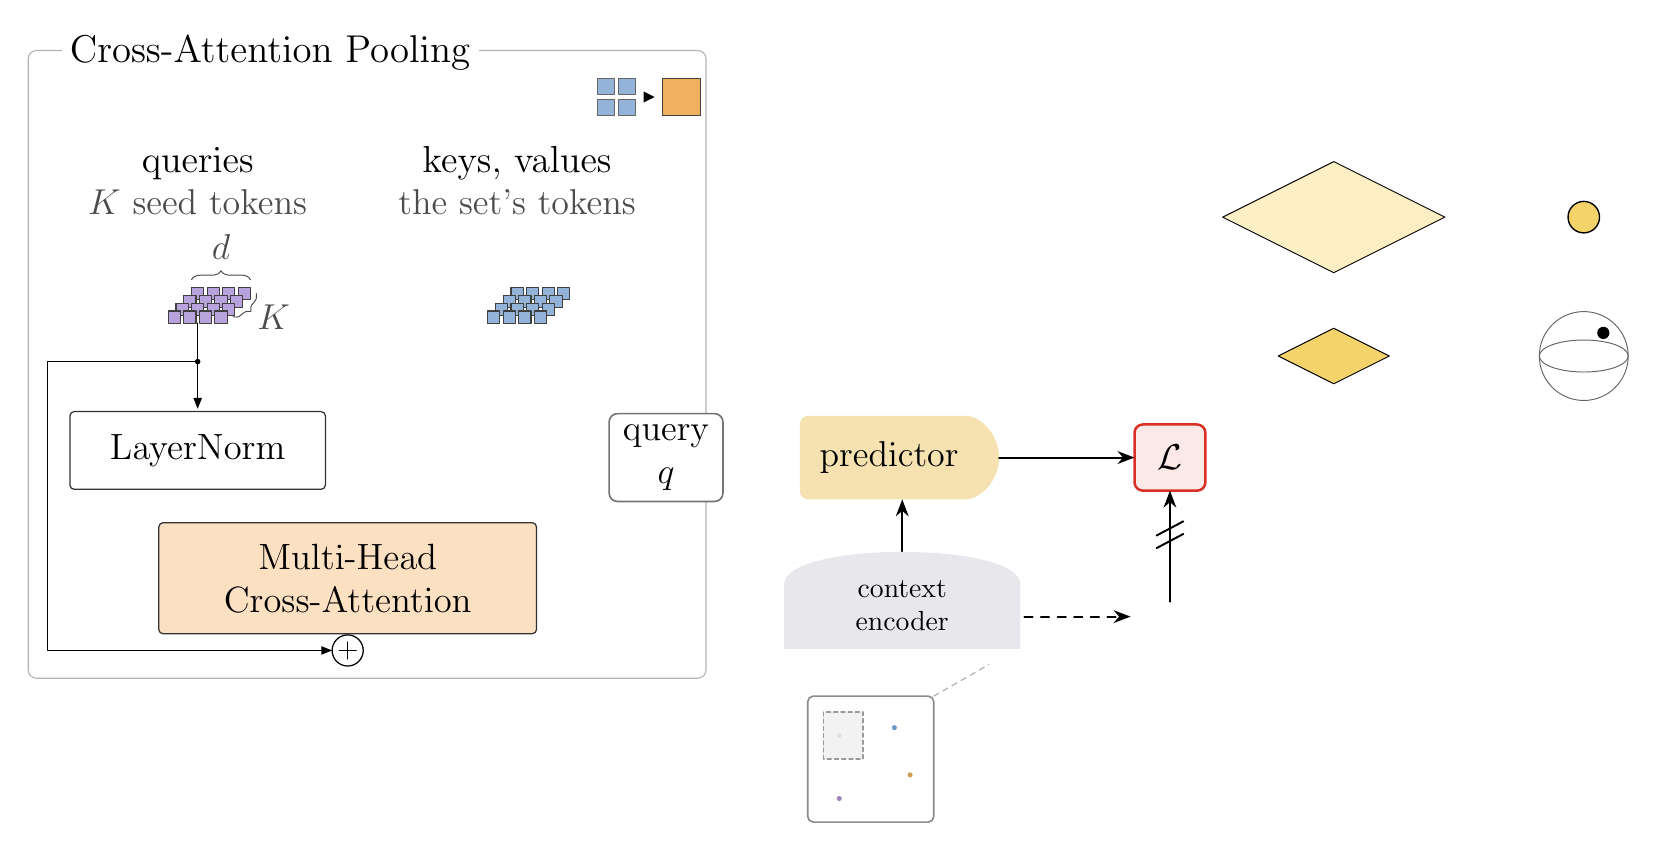
\begin{tikzpicture}[x=1bp, y=1bp, paper]
  % a card with its name on the border and a mini icon
  \card{0,0}{244}{226}{Cross-Attention Pooling}
  \minipool{205,-10}
  \twolevel{61,-44}{queries}{$K$ seed tokens}
  \twolevel{176,-44}{keys, values}{the set's tokens}
  \tokstack{61,-96}{tokpurple}
  \tokwidthbrace{61,-96}{$d$}
  \tokdepthbrace{61,-96}{$K$}
  \tokstack{176,-96}{tokblue}
  \node[box] (ln) at (61,-144) {LayerNorm};
  \draw[wire] (61,-98.2) -- (61,-129);
  \node[opbox] (att) at (115,-190) {Multi-Head\\Cross-Attention};
  \joincircle{115,-216}
  \coordinate (tap) at (61,-112); \coordinate (side) at (7,0); \coordinate (jn) at (115,-216);
  \residual{tap}{side}{jn}
  % overview family, in cm, beside the card
  \begin{scope}[x=1cm, y=1cm, shift={(9.6cm,-7.6cm)}]
    \slab{0,0}{3.0}{context\\encoder}
    \dcap{0.2,1.9}{2.0}{1.06}{predictor}
    \draw[flow] (1.5,1.24) -- (1.5,1.9);
    \node[qbox] at (-1.5,2.43) {query\\$q$};
    \node[loss] at (4.9,2.43) {$\mathcal{L}$};
    \draw[flow] (2.73,2.43) -- (4.45,2.43);
    \draw[ema] (3.05,0.41) -- (4.4,0.41);
    \draw[flowbare] (4.9,0.6) -- (4.9,1.2); \draw[flow] (4.9,1.2) -- (4.9,2.01);
    \stopgrad{4.9,1.45}
    \draw[crop] (0.3,-2.2) rectangle (1.9,-0.6);
    \draw[maskbox] (0.5,-1.4) rectangle (1.0,-0.8);
    \figpoint{1.4,-1.0}{ptblue} \figpoint{1.6,-1.6}{ptochre} \figpoint{0.7,-1.9}{ptpurple}
    \figmasked{0.7,-1.1}
    \draw[zoomlink] (1.9,-0.6) -- (2.6,-0.2);
  \end{scope}
  \isotile{470,-60}{40}{tilepale}
  \isotile{470,-110}{20}{tilestrong}
  \node[treenode, fill=tilestrong] at (560,-60) {};
  \unitsphere{560,-110}{16}
\end{tikzpicture}
\end{document}

%  and then has its own document environment with one tikzpicture. To
%  deliver, inline it (scripts/render_figure.py --inline OUT.tex copies
%  everything above the line "%%%% FIGURE BODY" into the file), so the
%  delivered figure needs no other file. The body below that line is a
%  smoke test that draws every element once; it makes this file compile
%  alone and is skipped when \figpreambleonly is defined.
%
%  Type: the TeX default, Computer Modern text and default math. fix-cm
%  allows arbitrary sizes. There is no font encoding package, no sans
%  text or math package, no mathastext and no lmodern here, and no sans
%  option: the author decided the font once ("make both figures default
%  tikz/tex font").
%
%  Colors are named by ROLE and defined once. A paper that needs another
%  value redefines that one name after this block (\definecolor{...});
%  that is the only knob. There is no theme switch.
%
%  Sizes are DESIGN sizes. The figures of this style are drawn large and
%  printed small (a card figure 850 bp wide printed at 388 bp, scale
%  0.457). Check the printed sizes with scripts/print_scale.py on the
%  compiled PDF; nothing may print under the 5 pt floor.
%
%  Units: generated figures and block cards use x=1bp, y=1bp (PDF big
%  points; a TeX point is 0.375 percent smaller, enough to slide a patch
%  off the artwork). Overviews and compositions use cm, as the source
%  figures did. Every macro below states its unit.
%
%  The \newcommand\fig... number lines are read by assets/figkit.py, so a
%  hand-written figure and a generated one share every size. Keep each
%  on one line in the form \newcommand\figName{number}.
%
%  Compile: pdflatex -interaction=nonstopmode -halt-on-error fig.tex
%  Needs: standalone, tikz, pgfplots (in a full TeX Live; BasicTeX needs
%  standalone and pgfplots added).
% =====================================================================
\documentclass[border=4pt]{standalone}
\usepackage{fix-cm}
\usepackage{amsmath,amssymb}
\usepackage{graphicx}
\usepackage{tikz}
\usetikzlibrary{arrows.meta,decorations.pathreplacing,calc}
\usepackage{pgfplots}
\pgfplotsset{compat=1.18}
\usepgfplotslibrary{fillbetween}

% ---------------------------------------------------------------------
%  NUMBERS (bp unless stated). Measured from the author's latest paper
%  figures with PyMuPDF; references/style.md gives the source of each.
% ---------------------------------------------------------------------
% block cards
\newcommand\figBoxW{92}        % every plain box (LayerNorm, FFN, ...)
\newcommand\figBoxH{28}
\newcommand\figOpW{136}        % the one operation box of a block
\newcommand\figOpH{40}
\newcommand\figBoxR{1.6}       % box corner radius
\newcommand\figCardR{3.0}      % card corner radius
\newcommand\figHeadL{3.9}      % flat-backed arrowhead, length
\newcommand\figHeadW{3.0}      % and width
\newcommand\figJoinR{5.6}      % join circle radius
\newcommand\figDotR{1.0}       % junction dot radius
\newcommand\figChip{4.4}       % one chip cell
\newcommand\figChipGap{1.2}    % gap between cells of a token
\newcommand\figChipCols{4}     % cells in a token row
\newcommand\figStackRows{4}    % rows in a K-deep stack
\newcommand\figStackOff{2.8}   % each row offset up and right by this
\newcommand\figMini{6.0}       % mini icon cell
\newcommand\figMiniGap{1.5}    % mini icon gap
\newcommand\figNameInset{12}   % card name starts this far right of the card edge
\newcommand\figNameDrop{0.32}  % card name baseline below the border, in units of its size
% line widths (TeX pt; 0.4 pt prints as the measured 0.3985 bp)
\newcommand\figLwCard{0.40}
\newcommand\figLwChip{0.40}
\newcommand\figLwWire{0.45}
\newcommand\figLwRes{0.40}
\newcommand\figLwMini{0.35}
\newcommand\figLwFlow{0.70}    % overview wires
\newcommand\figLwRail{0.60}    % feedback rails of a hierarchy
% type at design scale (TeX pt)
\newcommand\figPtName{14.0}    % card name on the border
\newcommand\figPtCap{13.6}     % stream captions, output caption, legend line
\newcommand\figPtBox{13.2}     % text inside boxes
\newcommand\figPtNote{13.0}    % gloss, wire labels, symbols beside glyphs
\newcommand\figPtLabel{13.0}   % overview labels
\newcommand\figPtSlab{10.0}    % two-line labels inside encoder slabs
\newcommand\figPtGloss{11.0}   % overview gloss
\newcommand\figPtTitle{16.0}   % composition panel title
\newcommand\figPtTile{13.5}    % label over a data tile
\newcommand\figPtCount{12.5}   % count or caption under a tile
\newcommand\figPtLetter{20.0}  % a bare panel letter (bold)

% font switches, one per role
\newcommand\fName{\fontsize{\figPtName}{16.8}\selectfont}
\newcommand\fCap{\fontsize{\figPtCap}{16.3}\selectfont}
\newcommand\fBox{\fontsize{\figPtBox}{15.8}\selectfont}
\newcommand\fNote{\fontsize{\figPtNote}{15.6}\selectfont}
\newcommand\fLabel{\fontsize{\figPtLabel}{15.6}\selectfont}
\newcommand\fSlab{\fontsize{\figPtSlab}{12}\selectfont}
\newcommand\fGloss{\fontsize{\figPtGloss}{13.2}\selectfont}
\newcommand\fTitle{\fontsize{\figPtTitle}{19.2}\selectfont}
\newcommand\fTile{\fontsize{\figPtTile}{16.2}\selectfont}
\newcommand\fCount{\fontsize{\figPtCount}{15}\selectfont}
\newcommand\fLetter{\fontsize{\figPtLetter}{24}\selectfont\bfseries}

% ---------------------------------------------------------------------
%  COLORS BY ROLE (hex measured from the paper figures)
% ---------------------------------------------------------------------
\colorlet{ink}{black}                       % wires and text
\colorlet{glossink}{black!70}               % secondary text: gloss, wire labels, symbols
\definecolor{boxline}{HTML}{333333}         % outline of every box
\definecolor{chipline}{HTML}{404040}        % outline of token chips
\definecolor{miniline}{HTML}{666666}        % outline of the what-it-does icon
\definecolor{cardline}{HTML}{B2B2B2}        % card frame
% token fills: a chip color names a KIND of token in every panel
\definecolor{tokblue}{HTML}{93B4D8}
\definecolor{tokorange}{HTML}{F0B060}
\definecolor{tokpurple}{HTML}{B9A3DC}
\definecolor{tokgreen}{HTML}{8FBFA0}
\definecolor{tokyellow}{HTML}{F5D36B}       % the leaf chips; also the selected path
% the one filled box of a block; every other box is white
\definecolor{oppeach}{HTML}{FBE0C2}         % cross-attention, pooling
\definecolor{opmint}{HTML}{D8E9DF}          % self-attention, neighborhood
\definecolor{opgray}{HTML}{E8E8E8}          % graph layer
% overview fills
\definecolor{slabgray}{HTML}{E8E8EC}        % encoder slab with a domed top
\definecolor{wheat}{HTML}{F5E2B0}           % predictor with a D-shaped cap
\definecolor{panelgray}{HTML}{F4F4F5}       % a faded module, shown but outside the claim
% the single loss box
\definecolor{lossline}{HTML}{D93025}
\definecolor{lossfill}{HTML}{FBE9E7}
% points, their density washes, graph edges
\definecolor{ptblue}{HTML}{5C8CC4}
\definecolor{ptochre}{HTML}{C98F3D}
\definecolor{ptpurple}{HTML}{9475B5}
\definecolor{washblue}{HTML}{A9C3E2}
\definecolor{washochre}{HTML}{E6D4AE}
\definecolor{washpurple}{HTML}{CDBBDF}
\colorlet{edgeline}{black!40}
% frames, masks, connectors, rules
\colorlet{cropline}{black!45}
\colorlet{queryline}{black!55}
\colorlet{zoomboxline}{black!75}
\colorlet{zoomline}{black!30}
\colorlet{maskline}{black!40}
\colorlet{maskfill}{black!5}
\colorlet{maskedpt}{black!13}
\colorlet{tileline}{black!28}
\colorlet{ruleline}{black!22}
% hierarchy
\definecolor{tilepale}{HTML}{FCEFC4}        % context tiles of the pyramid
\colorlet{tilestrong}{tokyellow}            % the selected path: tiles and tree nodes
\colorlet{treeedge}{black!55}
% sphere glyph
\colorlet{graticule}{black!22}
% sequential ramp of the package (data-figures RANK5): light to dark
\definecolor{ramp1}{HTML}{F1F6FF}
\definecolor{ramp2}{HTML}{C7DCFF}
\definecolor{ramp3}{HTML}{8FB9FF}
\definecolor{ramp4}{HTML}{4D97FF}
\definecolor{ramp5}{HTML}{003FBD}
% data plots: the package's color roles for compared items (data-figures style tokens)
\definecolor{hero}{HTML}{0072B2}            % the method the paper is about
\definecolor{rival}{HTML}{E69F00}           % the strongest comparator
\definecolor{othergray}{HTML}{A8A8AD}       % every other comparator
\definecolor{basegray}{HTML}{6E6E73}        % an untrained or trivial baseline
\definecolor{bandgray}{HTML}{EFEFF1}        % seed-to-seed noise band
\definecolor{guidegray}{HTML}{D1D1D6}       % guide lines and the grid of a heat matrix

% ---------------------------------------------------------------------
%  STYLES
% ---------------------------------------------------------------------
\tikzset{
  paper/.style={line cap=round, line join=round},
  every node/.append style={text=ink},
  % text
  gloss/.style={text=glossink},
  capt/.style={font=\fCap},
  note/.style={font=\fNote, text=glossink},
  lbl/.style={font=\fLabel, align=center},
  glossnote/.style={font=\fGloss, text=glossink, align=center},
  % boxes (bp): one size for every plain box, one for the operation box
  box/.style={draw=boxline, fill=white, line width=\figLwWire pt,
    rounded corners=\figBoxR bp, minimum width=\figBoxW bp, minimum height=\figBoxH bp,
    inner sep=0pt, outer sep=0pt, align=center, font=\fBox},
  opbox/.style={box, fill=#1, minimum width=\figOpW bp, minimum height=\figOpH bp},
  opbox/.default=oppeach,
  % wires (bp family): flat-backed head, stops 1 bp short of a box
  wire/.style={draw=ink, line width=\figLwWire pt,
    -{Triangle[length=\figHeadL bp, width=\figHeadW bp]}},
  wirebare/.style={draw=ink, line width=\figLwWire pt},
  resid/.style={draw=ink, line width=\figLwRes pt,
    -{Triangle[length=\figHeadL bp, width=\figHeadW bp]}},
  residbare/.style={draw=ink, line width=\figLwRes pt},
  chip/.style={draw=chipline, line width=\figLwChip pt},
  mini/.style={draw=miniline, line width=\figLwMini pt},
  bracegloss/.style={draw=glossink, line width=\figLwMini pt, decorate,
    decoration={brace, amplitude=3.2bp, raise=#1}},
  bracegloss/.default=1.4bp,
  % card frame and its name on the border
  card/.style={draw=cardline, line width=\figLwCard pt, rounded corners=\figCardR bp},
  cardname/.style={anchor=base west, fill=white, inner xsep=3bp, inner ysep=3bp,
    outer sep=0pt, font=\fName},
  % overview family (cm): wires, EMA, continuation
  flow/.style={draw=ink, line width=\figLwFlow pt, -{Stealth}},
  flowbare/.style={draw=ink, line width=\figLwFlow pt},
  ema/.style={flow, dashed},
  % hierarchy rails (bp family): Stealth heads as in the hierarchy panel
  rail/.style={draw=ink, line width=\figLwRail pt,
    -{Stealth[length=\figHeadL bp, width=2.9bp]}},
  railbare/.style={draw=ink, line width=\figLwRail pt},
  railcont/.style={rail, dash pattern=on 2.989bp off 2.989bp},
  railcontbare/.style={railbare, dash pattern=on 2.989bp off 2.989bp},
  % overview shapes (outer sep 0: an anchor such as (q.east) lies ON the frame line, so a wire drawn from it
  % starts on the frame and not half a line width outside it)
  qbox/.style={draw=queryline, line width=0.6pt, fill=white, rounded corners=3pt,
    inner xsep=5pt, inner ysep=4pt, outer sep=0pt, align=center, font=\fLabel},
  loss/.style={draw=lossline, line width=0.9pt, fill=lossfill, rounded corners=3pt,
    minimum width=0.90cm, minimum height=0.84cm, inner sep=0pt, outer sep=0pt, font=\fLabel},
  % crops, masks, zoom
  crop/.style={draw=cropline, line width=0.6pt, rounded corners=2pt, fill=white},
  maskbox/.style={draw=maskline, line width=0.6pt, dash pattern=on 1.4pt off 1.2pt,
    fill=maskfill},
  zoombox/.style={draw=zoomboxline, line width=0.55pt},
  zoomlink/.style={draw=zoomline, line width=0.45pt, dash pattern=on 2pt off 1.8pt},
  graphedge/.style={draw=edgeline, line width=0.34pt},
  % composition
  tileframe/.style={draw=tileline, line width=0.4pt},
  panelrule/.style={draw=ruleline, line width=0.4pt},
  paneltitle/.style={anchor=south west, inner sep=2pt, font=\fTitle, align=left},
  tilelabel/.style={font=\fTile, align=center},
  tilecount/.style={font=\fCount, align=center},
  % hierarchy: tree and pyramid
  treenode/.style={circle, draw=ink, line width=0.5pt, fill=white,
    minimum size=11.34bp, inner sep=0pt, outer sep=0pt},
  treeedge/.style={draw=treeedge, line width=0.5pt},
  treepath/.style={draw=ink, line width=1.1pt},
  isotile/.style={draw=ink, line width=0.35pt},
}

% ---------------------------------------------------------------------
%  MACROS (coordinates are any TikZ coordinate; offsets carry their unit)
% ---------------------------------------------------------------------
% a token: a row of #3 chip cells centered on #1, fill #2
\newcommand\tokrow[3]{%
  \pgfmathsetmacro\figRowW{#3*\figChip+(#3-1)*\figChipGap}%
  \pgfmathsetmacro\figHalfC{\figChip/2}%
  \foreach \kk in {1,...,#3}{%
    \pgfmathsetmacro\figCx{-\figRowW/2+(\kk-1)*(\figChip+\figChipGap)}%
    \draw[chip, fill=#2] ($(#1)+(\figCx bp,-\figHalfC bp)$) rectangle ++(\figChip bp,\figChip bp);
  }}
% a set of K tokens: [rows] rows of \figChipCols cells stacked behind one
% another, each row offset up and right; #1 is the FRONT row's center
\newcommand\tokstack[3][\figStackRows]{%
  \pgfmathtruncatemacro\figRm{#1-1}%
  \foreach \ii in {\figRm,...,0}{%
    \pgfmathsetmacro\figOff{\ii*\figStackOff}%
    \tokrow{$(#2)+(\figOff bp,\figOff bp)$}{#3}{\figChipCols}%
  }}
% the stack's width, bracketed over its BACK row (label #3, e.g. $d$)
\newcommand\tokwidthbrace[3][\figStackRows]{%
  \pgfmathsetmacro\figRowW{\figChipCols*\figChip+(\figChipCols-1)*\figChipGap}%
  \pgfmathsetmacro\figBx{(#1-1)*\figStackOff}%
  \pgfmathsetmacro\figTop{\figChip/2+(#1-1)*\figStackOff+1.5}%
  \draw[bracegloss] ($(#2)+(\figBx bp-\figRowW bp/2,\figTop bp)$)
      -- ($(#2)+(\figBx bp+\figRowW bp/2,\figTop bp)$);
  \node[note, anchor=base, inner sep=0pt] at ($(#2)+(\figBx bp,\figTop bp+8.5bp)$) {#3};}
% the stack's COUNT, bracketed along its own diagonal, drawn back to front
% so it bulges away from the stack (label #3, e.g. $K$)
\newcommand\tokdepthbrace[3][\figStackRows]{%
  \pgfmathsetmacro\figRowW{\figChipCols*\figChip+(\figChipCols-1)*\figChipGap}%
  \pgfmathsetmacro\figBk{(#1-1)*\figStackOff}%
  \pgfmathsetmacro\figD{2.2*0.7071}%
  \pgfmathsetmacro\figG{7.0*0.7071}%
  \coordinate (fig@back) at ($(#2)+(\figRowW bp/2+\figBk bp+\figD bp,\figChip bp/2+\figBk bp-\figD bp)$);
  \coordinate (fig@front) at ($(#2)+(\figRowW bp/2+\figD bp,\figChip bp/2-\figD bp)$);
  \draw[bracegloss=0.8bp] (fig@back) -- (fig@front);
  \node[note, anchor=base west, inner sep=0pt] at
    ($(fig@back)!0.5!(fig@front)+(\figG bp,-\figG bp-0.34*\figPtNote bp)$) {#3};}
% join circle with a plus: residual and other additions
\newcommand\joincircle[1]{%
  \draw[ink, fill=white, line width=\figLwWire pt] (#1) circle (\figJoinR bp);
  \pgfmathsetmacro\figArm{0.55*\figJoinR}%
  \draw[ink, line width=\figLwChip pt] ($(#1)+(-\figArm bp,0)$) -- ($(#1)+(\figArm bp,0)$);
  \draw[ink, line width=\figLwChip pt] ($(#1)+(0,-\figArm bp)$) -- ($(#1)+(0,\figArm bp)$);}
% junction dot: where a wire branches
\newcommand\junction[1]{\fill[ink] (#1) circle (\figDotR bp);}
% pre-norm residual: tap #1 (dot), run out to the x of #2, come back into
% the side of the join at #3 that faces the margin
\newcommand\residual[3]{%
  \junction{#1}
  \draw[resid] let \p1=(#2), \p2=(#3) in
    (#1) -- (#1 -| #2) -- (#3 -| #2) -- ($(#3)+({sign(\x1-\x2)*\figJoinR*1bp},0)$);}
% a card: frame with the name ON the top border (border masked by the
% name's own box); #1 top-left corner, #2 width and #3 height in bp
\newcommand\card[4]{%
  \draw[card] (#1) rectangle ++(#2 bp,-#3 bp);
  \pgfmathsetmacro\figNd{\figNameDrop*\figPtName}%
  \node[cardname] at ($(#1)+(\figNameInset bp,-\figNd bp)$) {#4};}
% a two-level label: a black name, its gray gloss 15 bp under it
\newcommand\twolevel[3]{%
  \node[capt, anchor=base, inner sep=0pt] at (#1) {#2};
  \node[note, anchor=base, inner sep=0pt] at ($(#1)+(0,-15bp)$) {#3};}
% mini icons, #1 = top-left corner. pool: four children to one parent
\newcommand\minipool[1]{%
  \pgfmathsetmacro\figP{\figMini+\figMiniGap}%
  \foreach \ii in {0,1}{\foreach \jj in {0,1}{%
    \draw[mini, fill=tokblue] ($(#1)+(\ii*\figP bp,-\jj*\figP bp)$) rectangle ++(\figMini bp,-\figMini bp);}}
  \pgfmathsetmacro\figH{2*\figP-\figMiniGap}%
  \fill[ink] ($(#1)+(\figH bp+3bp,-\figH bp/2+2bp)$) -- ++(4bp,-2bp) -- ++(-4bp,-2bp) -- cycle;
  \draw[chip, line width=\figLwMini pt, fill=tokorange] ($(#1)+(\figH bp+10bp,0)$) rectangle ++(\figH bp,-\figH bp);}
% mix: a tile and its neighborhood to that tile
\newcommand\minimix[1]{%
  \pgfmathsetmacro\figP{\figMini+\figMiniGap}%
  \foreach \ii in {0,1,2}{\foreach \jj in {0,1,2}{%
    \pgfmathsetmacro\figCtr{(\ii==1)&&(\jj==1)}%
    \ifdim\figCtr pt>0.5pt\def\figF{tokorange!70!black}\else\def\figF{tokorange}\fi
    \draw[mini, fill=\figF] ($(#1)+(\ii*\figP bp,-\jj*\figP bp)$) rectangle ++(\figMini bp,-\figMini bp);}}
  \pgfmathsetmacro\figH{3*\figP-\figMiniGap}%
  \fill[ink] ($(#1)+(\figH bp+3bp,-\figH bp/2+2bp)$) -- ++(4bp,-2bp) -- ++(-4bp,-2bp) -- cycle;
  \draw[mini, fill=tokblue] ($(#1)+(\figH bp+10bp,-\figP bp)$) rectangle ++(\figMini bp,-\figMini bp);}
% read: tiles coarse to fine to one point
\newcommand\miniread[1]{%
  \pgfmathsetmacro\figP{\figMini+\figMiniGap}%
  \foreach \ii in {0,1,2}{%
    \pgfmathsetmacro\figS{\figMini*(1-0.2*\ii)}%
    \draw[mini, fill=tokblue] ($(#1)+(\ii*\figP bp,-\figMini bp/2+\figS bp/2)$) rectangle ++(\figS bp,-\figS bp);}
  \pgfmathsetmacro\figXa{3*\figP-\figMiniGap+3}%
  \fill[ink] ($(#1)+(\figXa bp,-\figMini bp/2+2bp)$) -- ++(4bp,-2bp) -- ++(-4bp,-2bp) -- cycle;
  \fill[chipline] ($(#1)+(\figXa bp+9bp,-\figMini bp/2)$) circle (2.2bp);}
% the unit sphere glyph of a card: outline, equator, one unit vector's dot
\newcommand\unitsphere[2]{% #1 center, #2 radius in bp
  \draw[mini] (#1) circle (#2 bp);
  \draw[mini] (#1) ellipse ({#2 bp} and {0.36*#2 bp});
  \fill[ink] ($(#1)+(0.44*#2 bp,0.52*#2 bp)$) circle (2.2bp);}
% overview (cm): encoder slab with a domed top; #1 bottom-left, #2 width in cm
\newcommand\slab[3]{%
  \path[fill=slabgray] (#1) -- ++(#2 cm,0) -- ++(0,0.82cm)
     .. controls +(0,0.55cm) and +(0,0.55cm) .. ++(-#2 cm,0) -- cycle;
  \node[font=\fSlab, align=center] at ($(#1)+(#2 cm/2,0.55cm)$) {#3};}
% predictor with a D-shaped cap; #1 bottom-left, #2 straight width, #3 height (cm)
\newcommand\dcap[4]{%
  \path[rounded corners=3pt, fill=wheat] (#1) -- ++(#2 cm,0)
     arc[start angle=-90, end angle=90, radius=#3 cm/2] -- ++(-#2 cm,0) -- cycle;
  \node[lbl] at ($(#1)+(#2 cm/2+#3 cm/8,#3 cm/2)$) {#4};}
% stop-gradient: two short parallel slashes across a vertical wire at #1;
% [90] turns them for a horizontal wire
\newcommand\stopgrad[2][0]{%
  \begin{scope}[rotate around={#1:(#2)}]
    \draw[ink, line width=\figLwFlow pt] ($(#2)+(-0.17cm,-0.17cm)$) -- ++(0.34cm,0.18cm);
    \draw[ink, line width=\figLwFlow pt] ($(#2)+(-0.17cm,-0.01cm)$) -- ++(0.34cm,0.18cm);
  \end{scope}}
% points (cm family): a point, a masked point, a graph node
\newcommand\figpoint[2]{\fill[#2, opacity=0.9] (#1) circle (0.032cm);}
\newcommand\figmasked[1]{\fill[maskedpt] (#1) circle (0.028cm);}
\newcommand\fignode[2]{\fill[#2, opacity=0.9] (#1) circle (0.052cm);}
% hierarchy: an isometric tile, #1 center, #2 half-width (bp), #3 fill
\newcommand\isotile[3]{%
  \draw[isotile, fill=#3] ($(#1)+(-#2 bp,0)$) -- ($(#1)+(0,#2 bp/2)$)
     -- ($(#1)+(#2 bp,0)$) -- ($(#1)+(0,-#2 bp/2)$) -- cycle;}
% composition (cm): a raster tile with its hairline frame; #1 x, #2 y
% (center), #3 width in cm, #4 file
\newcommand\tile[4]{%
  \node[inner sep=0pt] at (#1,#2) {\includegraphics[width=#3cm]{#4}};
  \draw[tileframe] ({#1-#3/2},{#2-#3/2}) rectangle ({#1+#3/2},{#2+#3/2});}
% a panel title: bold letter, parenthesis, two spaces, a short name
\newcommand\paneltitle[3]{\node[paneltitle] at (#1) {\textbf{#2)}\ \ #3};}
% a bare panel letter (bold, one size and one baseline for every letter)
\newcommand\panelletter[2]{\node[anchor=base west, inner sep=0pt, font=\fLetter] at (#1) {#2};}

% ---------------------------------------------------------------------
%  PGFPLOTS: plots are drawn at their PRINTED size, so their type is the
%  package's on-page tiers (7 pt titles, 6 pt labels, 5 pt ticks).
% ---------------------------------------------------------------------
\pgfplotsset{
  paperaxis/.style={
    axis lines=left, axis line style={-, draw=black!93, line width=0.5pt},
    tick align=outside, tick style={draw=black!93, line width=0.4pt},
    major tick length=1.8pt, minor tick length=0pt,
    every tick label/.append style={font=\fontsize{5}{6}\selectfont},
    label style={font=\fontsize{6}{7.2}\selectfont},
    title style={font=\fontsize{7}{8.4}\selectfont, yshift=-2pt},
    every axis plot/.append style={line width=0.8pt},
    legend style={draw=none, fill=none, font=\fontsize{5}{6}\selectfont},
    clip=false, scale only axis,
  },
  colormap={rank5}{color=(ramp1) color=(ramp2) color=(ramp3) color=(ramp4) color=(ramp5)},
}

%%%% FIGURE BODY: the preamble ends above this line; below is the smoke test
\ifdefined\figpreambleonly\expandafter\endinput\fi
\begin{document}
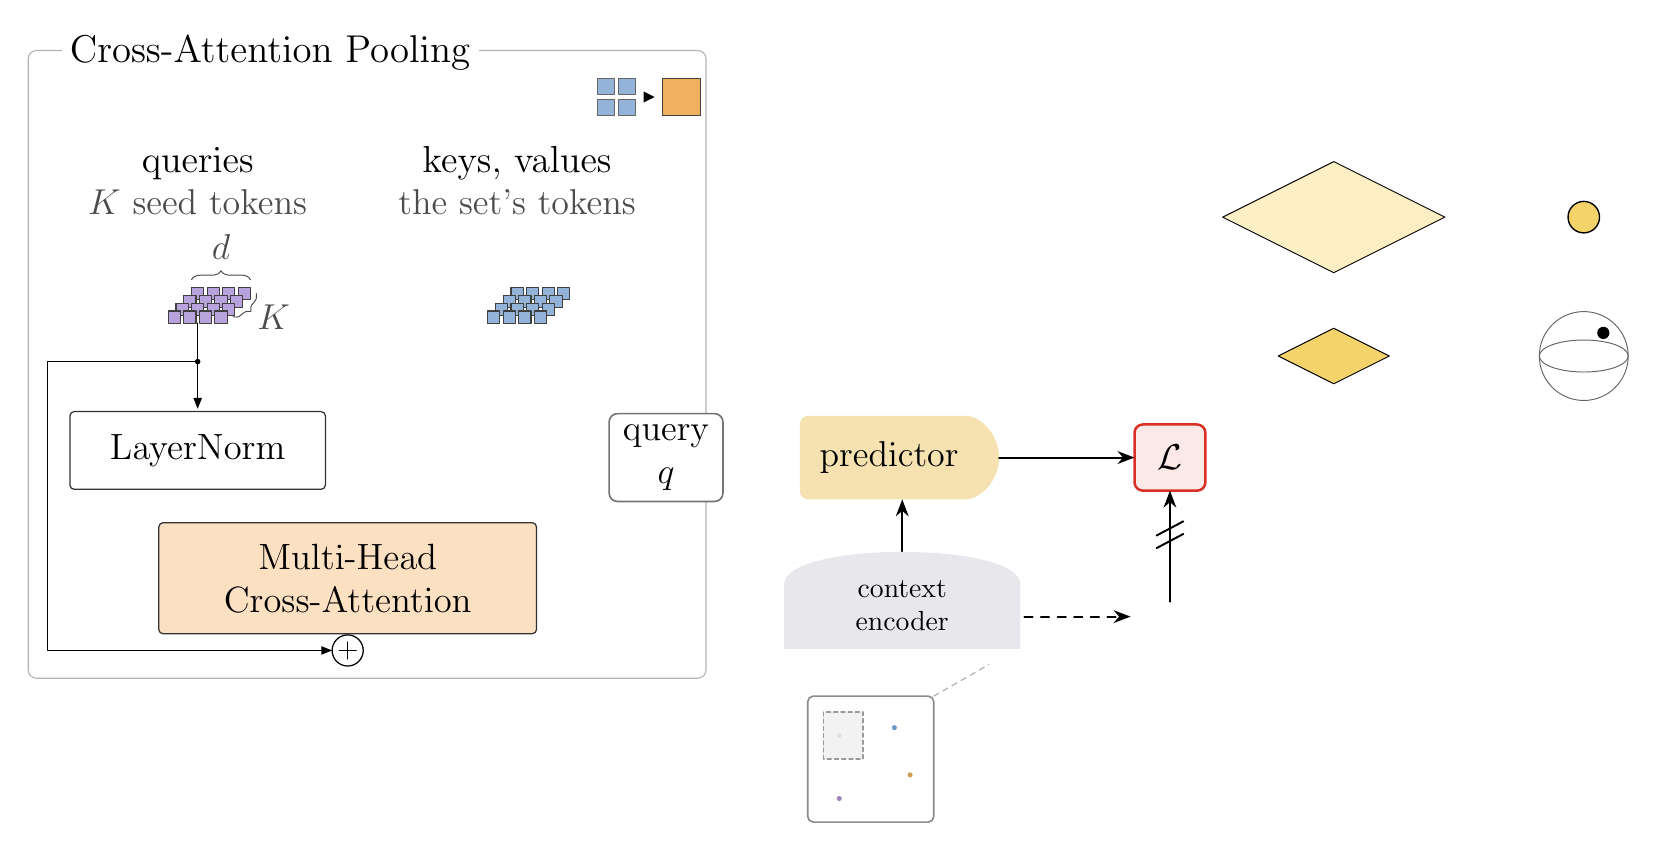
\begin{tikzpicture}[x=1bp, y=1bp, paper]
  % a card with its name on the border and a mini icon
  \card{0,0}{244}{226}{Cross-Attention Pooling}
  \minipool{205,-10}
  \twolevel{61,-44}{queries}{$K$ seed tokens}
  \twolevel{176,-44}{keys, values}{the set's tokens}
  \tokstack{61,-96}{tokpurple}
  \tokwidthbrace{61,-96}{$d$}
  \tokdepthbrace{61,-96}{$K$}
  \tokstack{176,-96}{tokblue}
  \node[box] (ln) at (61,-144) {LayerNorm};
  \draw[wire] (61,-98.2) -- (61,-129);
  \node[opbox] (att) at (115,-190) {Multi-Head\\Cross-Attention};
  \joincircle{115,-216}
  \coordinate (tap) at (61,-112); \coordinate (side) at (7,0); \coordinate (jn) at (115,-216);
  \residual{tap}{side}{jn}
  % overview family, in cm, beside the card
  \begin{scope}[x=1cm, y=1cm, shift={(9.6cm,-7.6cm)}]
    \slab{0,0}{3.0}{context\\encoder}
    \dcap{0.2,1.9}{2.0}{1.06}{predictor}
    \draw[flow] (1.5,1.24) -- (1.5,1.9);
    \node[qbox] at (-1.5,2.43) {query\\$q$};
    \node[loss] at (4.9,2.43) {$\mathcal{L}$};
    \draw[flow] (2.73,2.43) -- (4.45,2.43);
    \draw[ema] (3.05,0.41) -- (4.4,0.41);
    \draw[flowbare] (4.9,0.6) -- (4.9,1.2); \draw[flow] (4.9,1.2) -- (4.9,2.01);
    \stopgrad{4.9,1.45}
    \draw[crop] (0.3,-2.2) rectangle (1.9,-0.6);
    \draw[maskbox] (0.5,-1.4) rectangle (1.0,-0.8);
    \figpoint{1.4,-1.0}{ptblue} \figpoint{1.6,-1.6}{ptochre} \figpoint{0.7,-1.9}{ptpurple}
    \figmasked{0.7,-1.1}
    \draw[zoomlink] (1.9,-0.6) -- (2.6,-0.2);
  \end{scope}
  \isotile{470,-60}{40}{tilepale}
  \isotile{470,-110}{20}{tilestrong}
  \node[treenode, fill=tilestrong] at (560,-60) {};
  \unitsphere{560,-110}{16}
\end{tikzpicture}
\end{document}

%  and then has its own document environment with one tikzpicture. To
%  deliver, inline it (scripts/render_figure.py --inline OUT.tex copies
%  everything above the line "%%%% FIGURE BODY" into the file), so the
%  delivered figure needs no other file. The body below that line is a
%  smoke test that draws every element once; it makes this file compile
%  alone and is skipped when \figpreambleonly is defined.
%
%  Type: the TeX default, Computer Modern text and default math. fix-cm
%  allows arbitrary sizes. There is no font encoding package, no sans
%  text or math package, no mathastext and no lmodern here, and no sans
%  option: the author decided the font once ("make both figures default
%  tikz/tex font").
%
%  Colors are named by ROLE and defined once. A paper that needs another
%  value redefines that one name after this block (\definecolor{...});
%  that is the only knob. There is no theme switch.
%
%  Sizes are DESIGN sizes. The figures of this style are drawn large and
%  printed small (a card figure 850 bp wide printed at 388 bp, scale
%  0.457). Check the printed sizes with scripts/print_scale.py on the
%  compiled PDF; nothing may print under the 5 pt floor.
%
%  Units: generated figures and block cards use x=1bp, y=1bp (PDF big
%  points; a TeX point is 0.375 percent smaller, enough to slide a patch
%  off the artwork). Overviews and compositions use cm, as the source
%  figures did. Every macro below states its unit.
%
%  The \newcommand\fig... number lines are read by assets/figkit.py, so a
%  hand-written figure and a generated one share every size. Keep each
%  on one line in the form \newcommand\figName{number}.
%
%  Compile: pdflatex -interaction=nonstopmode -halt-on-error fig.tex
%  Needs: standalone, tikz, pgfplots (in a full TeX Live; BasicTeX needs
%  standalone and pgfplots added).
% =====================================================================
\documentclass[border=4pt]{standalone}
\usepackage{fix-cm}
\usepackage{amsmath,amssymb}
\usepackage{graphicx}
\usepackage{tikz}
\usetikzlibrary{arrows.meta,decorations.pathreplacing,calc}
\usepackage{pgfplots}
\pgfplotsset{compat=1.18}
\usepgfplotslibrary{fillbetween}

% ---------------------------------------------------------------------
%  NUMBERS (bp unless stated). Measured from the author's latest paper
%  figures with PyMuPDF; references/style.md gives the source of each.
% ---------------------------------------------------------------------
% block cards
\newcommand\figBoxW{92}        % every plain box (LayerNorm, FFN, ...)
\newcommand\figBoxH{28}
\newcommand\figOpW{136}        % the one operation box of a block
\newcommand\figOpH{40}
\newcommand\figBoxR{1.6}       % box corner radius
\newcommand\figCardR{3.0}      % card corner radius
\newcommand\figHeadL{3.9}      % flat-backed arrowhead, length
\newcommand\figHeadW{3.0}      % and width
\newcommand\figJoinR{5.6}      % join circle radius
\newcommand\figDotR{1.0}       % junction dot radius
\newcommand\figChip{4.4}       % one chip cell
\newcommand\figChipGap{1.2}    % gap between cells of a token
\newcommand\figChipCols{4}     % cells in a token row
\newcommand\figStackRows{4}    % rows in a K-deep stack
\newcommand\figStackOff{2.8}   % each row offset up and right by this
\newcommand\figMini{6.0}       % mini icon cell
\newcommand\figMiniGap{1.5}    % mini icon gap
\newcommand\figNameInset{12}   % card name starts this far right of the card edge
\newcommand\figNameDrop{0.32}  % card name baseline below the border, in units of its size
% line widths (TeX pt; 0.4 pt prints as the measured 0.3985 bp)
\newcommand\figLwCard{0.40}
\newcommand\figLwChip{0.40}
\newcommand\figLwWire{0.45}
\newcommand\figLwRes{0.40}
\newcommand\figLwMini{0.35}
\newcommand\figLwFlow{0.70}    % overview wires
\newcommand\figLwRail{0.60}    % feedback rails of a hierarchy
% type at design scale (TeX pt)
\newcommand\figPtName{14.0}    % card name on the border
\newcommand\figPtCap{13.6}     % stream captions, output caption, legend line
\newcommand\figPtBox{13.2}     % text inside boxes
\newcommand\figPtNote{13.0}    % gloss, wire labels, symbols beside glyphs
\newcommand\figPtLabel{13.0}   % overview labels
\newcommand\figPtSlab{10.0}    % two-line labels inside encoder slabs
\newcommand\figPtGloss{11.0}   % overview gloss
\newcommand\figPtTitle{16.0}   % composition panel title
\newcommand\figPtTile{13.5}    % label over a data tile
\newcommand\figPtCount{12.5}   % count or caption under a tile
\newcommand\figPtLetter{20.0}  % a bare panel letter (bold)

% font switches, one per role
\newcommand\fName{\fontsize{\figPtName}{16.8}\selectfont}
\newcommand\fCap{\fontsize{\figPtCap}{16.3}\selectfont}
\newcommand\fBox{\fontsize{\figPtBox}{15.8}\selectfont}
\newcommand\fNote{\fontsize{\figPtNote}{15.6}\selectfont}
\newcommand\fLabel{\fontsize{\figPtLabel}{15.6}\selectfont}
\newcommand\fSlab{\fontsize{\figPtSlab}{12}\selectfont}
\newcommand\fGloss{\fontsize{\figPtGloss}{13.2}\selectfont}
\newcommand\fTitle{\fontsize{\figPtTitle}{19.2}\selectfont}
\newcommand\fTile{\fontsize{\figPtTile}{16.2}\selectfont}
\newcommand\fCount{\fontsize{\figPtCount}{15}\selectfont}
\newcommand\fLetter{\fontsize{\figPtLetter}{24}\selectfont\bfseries}

% ---------------------------------------------------------------------
%  COLORS BY ROLE (hex measured from the paper figures)
% ---------------------------------------------------------------------
\colorlet{ink}{black}                       % wires and text
\colorlet{glossink}{black!70}               % secondary text: gloss, wire labels, symbols
\definecolor{boxline}{HTML}{333333}         % outline of every box
\definecolor{chipline}{HTML}{404040}        % outline of token chips
\definecolor{miniline}{HTML}{666666}        % outline of the what-it-does icon
\definecolor{cardline}{HTML}{B2B2B2}        % card frame
% token fills: a chip color names a KIND of token in every panel
\definecolor{tokblue}{HTML}{93B4D8}
\definecolor{tokorange}{HTML}{F0B060}
\definecolor{tokpurple}{HTML}{B9A3DC}
\definecolor{tokgreen}{HTML}{8FBFA0}
\definecolor{tokyellow}{HTML}{F5D36B}       % the leaf chips; also the selected path
% the one filled box of a block; every other box is white
\definecolor{oppeach}{HTML}{FBE0C2}         % cross-attention, pooling
\definecolor{opmint}{HTML}{D8E9DF}          % self-attention, neighborhood
\definecolor{opgray}{HTML}{E8E8E8}          % graph layer
% overview fills
\definecolor{slabgray}{HTML}{E8E8EC}        % encoder slab with a domed top
\definecolor{wheat}{HTML}{F5E2B0}           % predictor with a D-shaped cap
\definecolor{panelgray}{HTML}{F4F4F5}       % a faded module, shown but outside the claim
% the single loss box
\definecolor{lossline}{HTML}{D93025}
\definecolor{lossfill}{HTML}{FBE9E7}
% points, their density washes, graph edges
\definecolor{ptblue}{HTML}{5C8CC4}
\definecolor{ptochre}{HTML}{C98F3D}
\definecolor{ptpurple}{HTML}{9475B5}
\definecolor{washblue}{HTML}{A9C3E2}
\definecolor{washochre}{HTML}{E6D4AE}
\definecolor{washpurple}{HTML}{CDBBDF}
\colorlet{edgeline}{black!40}
% frames, masks, connectors, rules
\colorlet{cropline}{black!45}
\colorlet{queryline}{black!55}
\colorlet{zoomboxline}{black!75}
\colorlet{zoomline}{black!30}
\colorlet{maskline}{black!40}
\colorlet{maskfill}{black!5}
\colorlet{maskedpt}{black!13}
\colorlet{tileline}{black!28}
\colorlet{ruleline}{black!22}
% hierarchy
\definecolor{tilepale}{HTML}{FCEFC4}        % context tiles of the pyramid
\colorlet{tilestrong}{tokyellow}            % the selected path: tiles and tree nodes
\colorlet{treeedge}{black!55}
% sphere glyph
\colorlet{graticule}{black!22}
% sequential ramp of the package (data-figures RANK5): light to dark
\definecolor{ramp1}{HTML}{F1F6FF}
\definecolor{ramp2}{HTML}{C7DCFF}
\definecolor{ramp3}{HTML}{8FB9FF}
\definecolor{ramp4}{HTML}{4D97FF}
\definecolor{ramp5}{HTML}{003FBD}
% data plots: the package's color roles for compared items (data-figures style tokens)
\definecolor{hero}{HTML}{0072B2}            % the method the paper is about
\definecolor{rival}{HTML}{E69F00}           % the strongest comparator
\definecolor{othergray}{HTML}{A8A8AD}       % every other comparator
\definecolor{basegray}{HTML}{6E6E73}        % an untrained or trivial baseline
\definecolor{bandgray}{HTML}{EFEFF1}        % seed-to-seed noise band
\definecolor{guidegray}{HTML}{D1D1D6}       % guide lines and the grid of a heat matrix

% ---------------------------------------------------------------------
%  STYLES
% ---------------------------------------------------------------------
\tikzset{
  paper/.style={line cap=round, line join=round},
  every node/.append style={text=ink},
  % text
  gloss/.style={text=glossink},
  capt/.style={font=\fCap},
  note/.style={font=\fNote, text=glossink},
  lbl/.style={font=\fLabel, align=center},
  glossnote/.style={font=\fGloss, text=glossink, align=center},
  % boxes (bp): one size for every plain box, one for the operation box
  box/.style={draw=boxline, fill=white, line width=\figLwWire pt,
    rounded corners=\figBoxR bp, minimum width=\figBoxW bp, minimum height=\figBoxH bp,
    inner sep=0pt, outer sep=0pt, align=center, font=\fBox},
  opbox/.style={box, fill=#1, minimum width=\figOpW bp, minimum height=\figOpH bp},
  opbox/.default=oppeach,
  % wires (bp family): flat-backed head, stops 1 bp short of a box
  wire/.style={draw=ink, line width=\figLwWire pt,
    -{Triangle[length=\figHeadL bp, width=\figHeadW bp]}},
  wirebare/.style={draw=ink, line width=\figLwWire pt},
  resid/.style={draw=ink, line width=\figLwRes pt,
    -{Triangle[length=\figHeadL bp, width=\figHeadW bp]}},
  residbare/.style={draw=ink, line width=\figLwRes pt},
  chip/.style={draw=chipline, line width=\figLwChip pt},
  mini/.style={draw=miniline, line width=\figLwMini pt},
  bracegloss/.style={draw=glossink, line width=\figLwMini pt, decorate,
    decoration={brace, amplitude=3.2bp, raise=#1}},
  bracegloss/.default=1.4bp,
  % card frame and its name on the border
  card/.style={draw=cardline, line width=\figLwCard pt, rounded corners=\figCardR bp},
  cardname/.style={anchor=base west, fill=white, inner xsep=3bp, inner ysep=3bp,
    outer sep=0pt, font=\fName},
  % overview family (cm): wires, EMA, continuation
  flow/.style={draw=ink, line width=\figLwFlow pt, -{Stealth}},
  flowbare/.style={draw=ink, line width=\figLwFlow pt},
  ema/.style={flow, dashed},
  % hierarchy rails (bp family): Stealth heads as in the hierarchy panel
  rail/.style={draw=ink, line width=\figLwRail pt,
    -{Stealth[length=\figHeadL bp, width=2.9bp]}},
  railbare/.style={draw=ink, line width=\figLwRail pt},
  railcont/.style={rail, dash pattern=on 2.989bp off 2.989bp},
  railcontbare/.style={railbare, dash pattern=on 2.989bp off 2.989bp},
  % overview shapes (outer sep 0: an anchor such as (q.east) lies ON the frame line, so a wire drawn from it
  % starts on the frame and not half a line width outside it)
  qbox/.style={draw=queryline, line width=0.6pt, fill=white, rounded corners=3pt,
    inner xsep=5pt, inner ysep=4pt, outer sep=0pt, align=center, font=\fLabel},
  loss/.style={draw=lossline, line width=0.9pt, fill=lossfill, rounded corners=3pt,
    minimum width=0.90cm, minimum height=0.84cm, inner sep=0pt, outer sep=0pt, font=\fLabel},
  % crops, masks, zoom
  crop/.style={draw=cropline, line width=0.6pt, rounded corners=2pt, fill=white},
  maskbox/.style={draw=maskline, line width=0.6pt, dash pattern=on 1.4pt off 1.2pt,
    fill=maskfill},
  zoombox/.style={draw=zoomboxline, line width=0.55pt},
  zoomlink/.style={draw=zoomline, line width=0.45pt, dash pattern=on 2pt off 1.8pt},
  graphedge/.style={draw=edgeline, line width=0.34pt},
  % composition
  tileframe/.style={draw=tileline, line width=0.4pt},
  panelrule/.style={draw=ruleline, line width=0.4pt},
  paneltitle/.style={anchor=south west, inner sep=2pt, font=\fTitle, align=left},
  tilelabel/.style={font=\fTile, align=center},
  tilecount/.style={font=\fCount, align=center},
  % hierarchy: tree and pyramid
  treenode/.style={circle, draw=ink, line width=0.5pt, fill=white,
    minimum size=11.34bp, inner sep=0pt, outer sep=0pt},
  treeedge/.style={draw=treeedge, line width=0.5pt},
  treepath/.style={draw=ink, line width=1.1pt},
  isotile/.style={draw=ink, line width=0.35pt},
}

% ---------------------------------------------------------------------
%  MACROS (coordinates are any TikZ coordinate; offsets carry their unit)
% ---------------------------------------------------------------------
% a token: a row of #3 chip cells centered on #1, fill #2
\newcommand\tokrow[3]{%
  \pgfmathsetmacro\figRowW{#3*\figChip+(#3-1)*\figChipGap}%
  \pgfmathsetmacro\figHalfC{\figChip/2}%
  \foreach \kk in {1,...,#3}{%
    \pgfmathsetmacro\figCx{-\figRowW/2+(\kk-1)*(\figChip+\figChipGap)}%
    \draw[chip, fill=#2] ($(#1)+(\figCx bp,-\figHalfC bp)$) rectangle ++(\figChip bp,\figChip bp);
  }}
% a set of K tokens: [rows] rows of \figChipCols cells stacked behind one
% another, each row offset up and right; #1 is the FRONT row's center
\newcommand\tokstack[3][\figStackRows]{%
  \pgfmathtruncatemacro\figRm{#1-1}%
  \foreach \ii in {\figRm,...,0}{%
    \pgfmathsetmacro\figOff{\ii*\figStackOff}%
    \tokrow{$(#2)+(\figOff bp,\figOff bp)$}{#3}{\figChipCols}%
  }}
% the stack's width, bracketed over its BACK row (label #3, e.g. $d$)
\newcommand\tokwidthbrace[3][\figStackRows]{%
  \pgfmathsetmacro\figRowW{\figChipCols*\figChip+(\figChipCols-1)*\figChipGap}%
  \pgfmathsetmacro\figBx{(#1-1)*\figStackOff}%
  \pgfmathsetmacro\figTop{\figChip/2+(#1-1)*\figStackOff+1.5}%
  \draw[bracegloss] ($(#2)+(\figBx bp-\figRowW bp/2,\figTop bp)$)
      -- ($(#2)+(\figBx bp+\figRowW bp/2,\figTop bp)$);
  \node[note, anchor=base, inner sep=0pt] at ($(#2)+(\figBx bp,\figTop bp+8.5bp)$) {#3};}
% the stack's COUNT, bracketed along its own diagonal, drawn back to front
% so it bulges away from the stack (label #3, e.g. $K$)
\newcommand\tokdepthbrace[3][\figStackRows]{%
  \pgfmathsetmacro\figRowW{\figChipCols*\figChip+(\figChipCols-1)*\figChipGap}%
  \pgfmathsetmacro\figBk{(#1-1)*\figStackOff}%
  \pgfmathsetmacro\figD{2.2*0.7071}%
  \pgfmathsetmacro\figG{7.0*0.7071}%
  \coordinate (fig@back) at ($(#2)+(\figRowW bp/2+\figBk bp+\figD bp,\figChip bp/2+\figBk bp-\figD bp)$);
  \coordinate (fig@front) at ($(#2)+(\figRowW bp/2+\figD bp,\figChip bp/2-\figD bp)$);
  \draw[bracegloss=0.8bp] (fig@back) -- (fig@front);
  \node[note, anchor=base west, inner sep=0pt] at
    ($(fig@back)!0.5!(fig@front)+(\figG bp,-\figG bp-0.34*\figPtNote bp)$) {#3};}
% join circle with a plus: residual and other additions
\newcommand\joincircle[1]{%
  \draw[ink, fill=white, line width=\figLwWire pt] (#1) circle (\figJoinR bp);
  \pgfmathsetmacro\figArm{0.55*\figJoinR}%
  \draw[ink, line width=\figLwChip pt] ($(#1)+(-\figArm bp,0)$) -- ($(#1)+(\figArm bp,0)$);
  \draw[ink, line width=\figLwChip pt] ($(#1)+(0,-\figArm bp)$) -- ($(#1)+(0,\figArm bp)$);}
% junction dot: where a wire branches
\newcommand\junction[1]{\fill[ink] (#1) circle (\figDotR bp);}
% pre-norm residual: tap #1 (dot), run out to the x of #2, come back into
% the side of the join at #3 that faces the margin
\newcommand\residual[3]{%
  \junction{#1}
  \draw[resid] let \p1=(#2), \p2=(#3) in
    (#1) -- (#1 -| #2) -- (#3 -| #2) -- ($(#3)+({sign(\x1-\x2)*\figJoinR*1bp},0)$);}
% a card: frame with the name ON the top border (border masked by the
% name's own box); #1 top-left corner, #2 width and #3 height in bp
\newcommand\card[4]{%
  \draw[card] (#1) rectangle ++(#2 bp,-#3 bp);
  \pgfmathsetmacro\figNd{\figNameDrop*\figPtName}%
  \node[cardname] at ($(#1)+(\figNameInset bp,-\figNd bp)$) {#4};}
% a two-level label: a black name, its gray gloss 15 bp under it
\newcommand\twolevel[3]{%
  \node[capt, anchor=base, inner sep=0pt] at (#1) {#2};
  \node[note, anchor=base, inner sep=0pt] at ($(#1)+(0,-15bp)$) {#3};}
% mini icons, #1 = top-left corner. pool: four children to one parent
\newcommand\minipool[1]{%
  \pgfmathsetmacro\figP{\figMini+\figMiniGap}%
  \foreach \ii in {0,1}{\foreach \jj in {0,1}{%
    \draw[mini, fill=tokblue] ($(#1)+(\ii*\figP bp,-\jj*\figP bp)$) rectangle ++(\figMini bp,-\figMini bp);}}
  \pgfmathsetmacro\figH{2*\figP-\figMiniGap}%
  \fill[ink] ($(#1)+(\figH bp+3bp,-\figH bp/2+2bp)$) -- ++(4bp,-2bp) -- ++(-4bp,-2bp) -- cycle;
  \draw[chip, line width=\figLwMini pt, fill=tokorange] ($(#1)+(\figH bp+10bp,0)$) rectangle ++(\figH bp,-\figH bp);}
% mix: a tile and its neighborhood to that tile
\newcommand\minimix[1]{%
  \pgfmathsetmacro\figP{\figMini+\figMiniGap}%
  \foreach \ii in {0,1,2}{\foreach \jj in {0,1,2}{%
    \pgfmathsetmacro\figCtr{(\ii==1)&&(\jj==1)}%
    \ifdim\figCtr pt>0.5pt\def\figF{tokorange!70!black}\else\def\figF{tokorange}\fi
    \draw[mini, fill=\figF] ($(#1)+(\ii*\figP bp,-\jj*\figP bp)$) rectangle ++(\figMini bp,-\figMini bp);}}
  \pgfmathsetmacro\figH{3*\figP-\figMiniGap}%
  \fill[ink] ($(#1)+(\figH bp+3bp,-\figH bp/2+2bp)$) -- ++(4bp,-2bp) -- ++(-4bp,-2bp) -- cycle;
  \draw[mini, fill=tokblue] ($(#1)+(\figH bp+10bp,-\figP bp)$) rectangle ++(\figMini bp,-\figMini bp);}
% read: tiles coarse to fine to one point
\newcommand\miniread[1]{%
  \pgfmathsetmacro\figP{\figMini+\figMiniGap}%
  \foreach \ii in {0,1,2}{%
    \pgfmathsetmacro\figS{\figMini*(1-0.2*\ii)}%
    \draw[mini, fill=tokblue] ($(#1)+(\ii*\figP bp,-\figMini bp/2+\figS bp/2)$) rectangle ++(\figS bp,-\figS bp);}
  \pgfmathsetmacro\figXa{3*\figP-\figMiniGap+3}%
  \fill[ink] ($(#1)+(\figXa bp,-\figMini bp/2+2bp)$) -- ++(4bp,-2bp) -- ++(-4bp,-2bp) -- cycle;
  \fill[chipline] ($(#1)+(\figXa bp+9bp,-\figMini bp/2)$) circle (2.2bp);}
% the unit sphere glyph of a card: outline, equator, one unit vector's dot
\newcommand\unitsphere[2]{% #1 center, #2 radius in bp
  \draw[mini] (#1) circle (#2 bp);
  \draw[mini] (#1) ellipse ({#2 bp} and {0.36*#2 bp});
  \fill[ink] ($(#1)+(0.44*#2 bp,0.52*#2 bp)$) circle (2.2bp);}
% overview (cm): encoder slab with a domed top; #1 bottom-left, #2 width in cm
\newcommand\slab[3]{%
  \path[fill=slabgray] (#1) -- ++(#2 cm,0) -- ++(0,0.82cm)
     .. controls +(0,0.55cm) and +(0,0.55cm) .. ++(-#2 cm,0) -- cycle;
  \node[font=\fSlab, align=center] at ($(#1)+(#2 cm/2,0.55cm)$) {#3};}
% predictor with a D-shaped cap; #1 bottom-left, #2 straight width, #3 height (cm)
\newcommand\dcap[4]{%
  \path[rounded corners=3pt, fill=wheat] (#1) -- ++(#2 cm,0)
     arc[start angle=-90, end angle=90, radius=#3 cm/2] -- ++(-#2 cm,0) -- cycle;
  \node[lbl] at ($(#1)+(#2 cm/2+#3 cm/8,#3 cm/2)$) {#4};}
% stop-gradient: two short parallel slashes across a vertical wire at #1;
% [90] turns them for a horizontal wire
\newcommand\stopgrad[2][0]{%
  \begin{scope}[rotate around={#1:(#2)}]
    \draw[ink, line width=\figLwFlow pt] ($(#2)+(-0.17cm,-0.17cm)$) -- ++(0.34cm,0.18cm);
    \draw[ink, line width=\figLwFlow pt] ($(#2)+(-0.17cm,-0.01cm)$) -- ++(0.34cm,0.18cm);
  \end{scope}}
% points (cm family): a point, a masked point, a graph node
\newcommand\figpoint[2]{\fill[#2, opacity=0.9] (#1) circle (0.032cm);}
\newcommand\figmasked[1]{\fill[maskedpt] (#1) circle (0.028cm);}
\newcommand\fignode[2]{\fill[#2, opacity=0.9] (#1) circle (0.052cm);}
% hierarchy: an isometric tile, #1 center, #2 half-width (bp), #3 fill
\newcommand\isotile[3]{%
  \draw[isotile, fill=#3] ($(#1)+(-#2 bp,0)$) -- ($(#1)+(0,#2 bp/2)$)
     -- ($(#1)+(#2 bp,0)$) -- ($(#1)+(0,-#2 bp/2)$) -- cycle;}
% composition (cm): a raster tile with its hairline frame; #1 x, #2 y
% (center), #3 width in cm, #4 file
\newcommand\tile[4]{%
  \node[inner sep=0pt] at (#1,#2) {\includegraphics[width=#3cm]{#4}};
  \draw[tileframe] ({#1-#3/2},{#2-#3/2}) rectangle ({#1+#3/2},{#2+#3/2});}
% a panel title: bold letter, parenthesis, two spaces, a short name
\newcommand\paneltitle[3]{\node[paneltitle] at (#1) {\textbf{#2)}\ \ #3};}
% a bare panel letter (bold, one size and one baseline for every letter)
\newcommand\panelletter[2]{\node[anchor=base west, inner sep=0pt, font=\fLetter] at (#1) {#2};}

% ---------------------------------------------------------------------
%  PGFPLOTS: plots are drawn at their PRINTED size, so their type is the
%  package's on-page tiers (7 pt titles, 6 pt labels, 5 pt ticks).
% ---------------------------------------------------------------------
\pgfplotsset{
  paperaxis/.style={
    axis lines=left, axis line style={-, draw=black!93, line width=0.5pt},
    tick align=outside, tick style={draw=black!93, line width=0.4pt},
    major tick length=1.8pt, minor tick length=0pt,
    every tick label/.append style={font=\fontsize{5}{6}\selectfont},
    label style={font=\fontsize{6}{7.2}\selectfont},
    title style={font=\fontsize{7}{8.4}\selectfont, yshift=-2pt},
    every axis plot/.append style={line width=0.8pt},
    legend style={draw=none, fill=none, font=\fontsize{5}{6}\selectfont},
    clip=false, scale only axis,
  },
  colormap={rank5}{color=(ramp1) color=(ramp2) color=(ramp3) color=(ramp4) color=(ramp5)},
}

%%%% FIGURE BODY: the preamble ends above this line; below is the smoke test
\ifdefined\figpreambleonly\expandafter\endinput\fi
\begin{document}
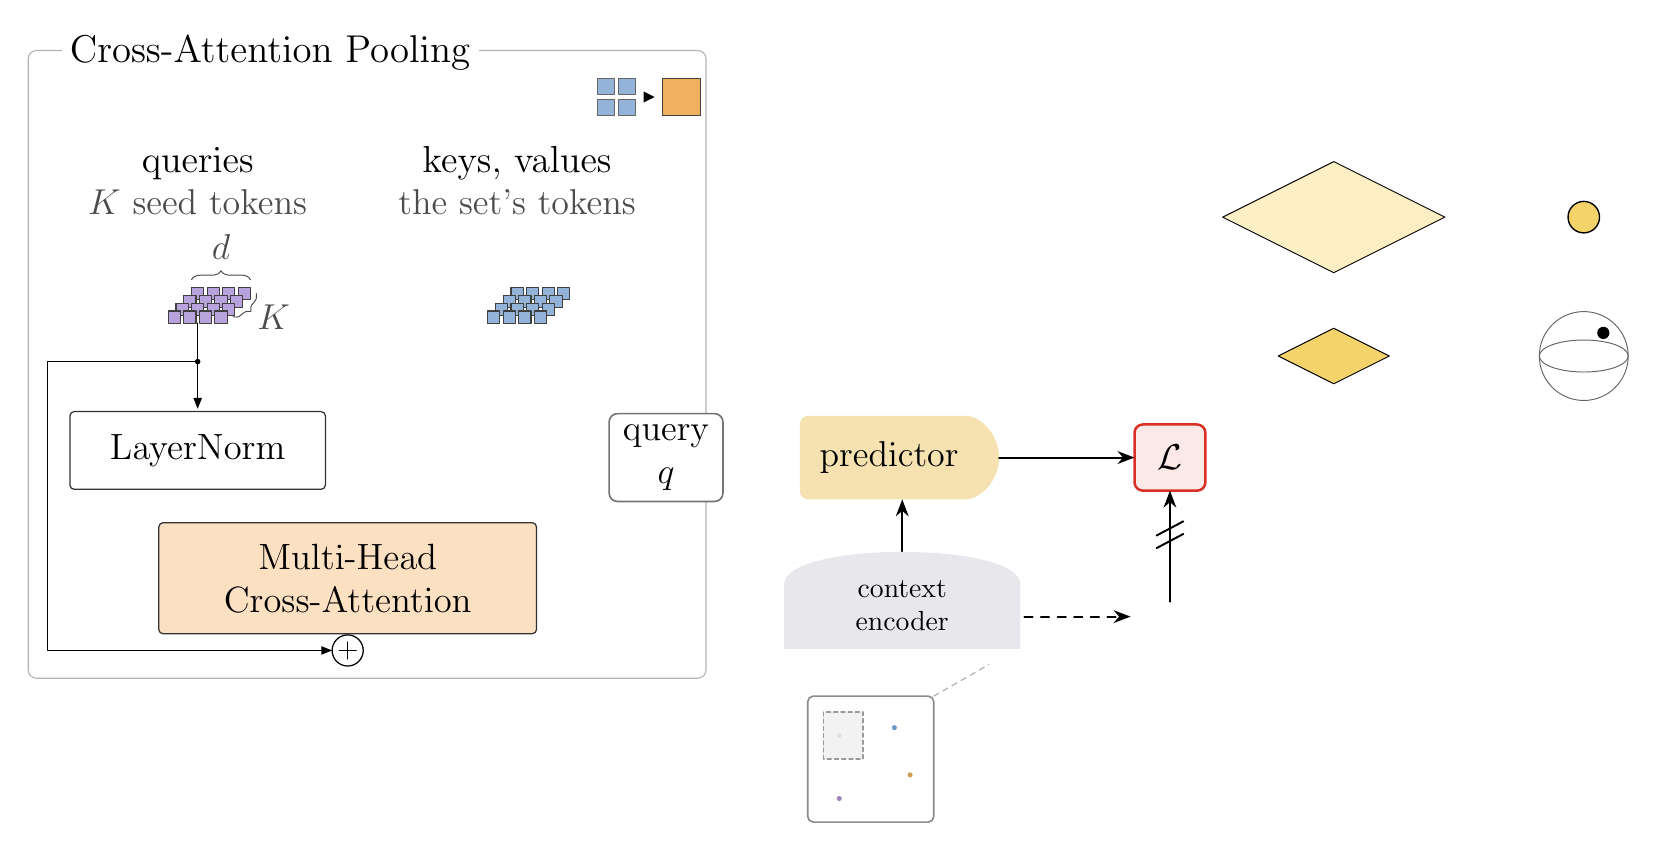
\begin{tikzpicture}[x=1bp, y=1bp, paper]
  % a card with its name on the border and a mini icon
  \card{0,0}{244}{226}{Cross-Attention Pooling}
  \minipool{205,-10}
  \twolevel{61,-44}{queries}{$K$ seed tokens}
  \twolevel{176,-44}{keys, values}{the set's tokens}
  \tokstack{61,-96}{tokpurple}
  \tokwidthbrace{61,-96}{$d$}
  \tokdepthbrace{61,-96}{$K$}
  \tokstack{176,-96}{tokblue}
  \node[box] (ln) at (61,-144) {LayerNorm};
  \draw[wire] (61,-98.2) -- (61,-129);
  \node[opbox] (att) at (115,-190) {Multi-Head\\Cross-Attention};
  \joincircle{115,-216}
  \coordinate (tap) at (61,-112); \coordinate (side) at (7,0); \coordinate (jn) at (115,-216);
  \residual{tap}{side}{jn}
  % overview family, in cm, beside the card
  \begin{scope}[x=1cm, y=1cm, shift={(9.6cm,-7.6cm)}]
    \slab{0,0}{3.0}{context\\encoder}
    \dcap{0.2,1.9}{2.0}{1.06}{predictor}
    \draw[flow] (1.5,1.24) -- (1.5,1.9);
    \node[qbox] at (-1.5,2.43) {query\\$q$};
    \node[loss] at (4.9,2.43) {$\mathcal{L}$};
    \draw[flow] (2.73,2.43) -- (4.45,2.43);
    \draw[ema] (3.05,0.41) -- (4.4,0.41);
    \draw[flowbare] (4.9,0.6) -- (4.9,1.2); \draw[flow] (4.9,1.2) -- (4.9,2.01);
    \stopgrad{4.9,1.45}
    \draw[crop] (0.3,-2.2) rectangle (1.9,-0.6);
    \draw[maskbox] (0.5,-1.4) rectangle (1.0,-0.8);
    \figpoint{1.4,-1.0}{ptblue} \figpoint{1.6,-1.6}{ptochre} \figpoint{0.7,-1.9}{ptpurple}
    \figmasked{0.7,-1.1}
    \draw[zoomlink] (1.9,-0.6) -- (2.6,-0.2);
  \end{scope}
  \isotile{470,-60}{40}{tilepale}
  \isotile{470,-110}{20}{tilestrong}
  \node[treenode, fill=tilestrong] at (560,-60) {};
  \unitsphere{560,-110}{16}
\end{tikzpicture}
\end{document}

%  and then has its own document environment with one tikzpicture. To
%  deliver, inline it (scripts/render_figure.py --inline OUT.tex copies
%  everything above the line "%%%% FIGURE BODY" into the file), so the
%  delivered figure needs no other file. The body below that line is a
%  smoke test that draws every element once; it makes this file compile
%  alone and is skipped when \figpreambleonly is defined.
%
%  Type: the TeX default, Computer Modern text and default math. fix-cm
%  allows arbitrary sizes. There is no font encoding package, no sans
%  text or math package, no mathastext and no lmodern here, and no sans
%  option: the author decided the font once ("make both figures default
%  tikz/tex font").
%
%  Colors are named by ROLE and defined once. A paper that needs another
%  value redefines that one name after this block (\definecolor{...});
%  that is the only knob. There is no theme switch.
%
%  Sizes are DESIGN sizes. The figures of this style are drawn large and
%  printed small (a card figure 850 bp wide printed at 388 bp, scale
%  0.457). Check the printed sizes with scripts/print_scale.py on the
%  compiled PDF; nothing may print under the 5 pt floor.
%
%  Units: generated figures and block cards use x=1bp, y=1bp (PDF big
%  points; a TeX point is 0.375 percent smaller, enough to slide a patch
%  off the artwork). Overviews and compositions use cm, as the source
%  figures did. Every macro below states its unit.
%
%  The \newcommand\fig... number lines are read by assets/figkit.py, so a
%  hand-written figure and a generated one share every size. Keep each
%  on one line in the form \newcommand\figName{number}.
%
%  Compile: pdflatex -interaction=nonstopmode -halt-on-error fig.tex
%  Needs: standalone, tikz, pgfplots (in a full TeX Live; BasicTeX needs
%  standalone and pgfplots added).
% =====================================================================
\documentclass[border=4pt]{standalone}
\usepackage{fix-cm}
\usepackage{amsmath,amssymb}
\usepackage{graphicx}
\usepackage{tikz}
\usetikzlibrary{arrows.meta,decorations.pathreplacing,calc}
\usepackage{pgfplots}
\pgfplotsset{compat=1.18}
\usepgfplotslibrary{fillbetween}

% ---------------------------------------------------------------------
%  NUMBERS (bp unless stated). Measured from the author's latest paper
%  figures with PyMuPDF; references/style.md gives the source of each.
% ---------------------------------------------------------------------
% block cards
\newcommand\figBoxW{92}        % every plain box (LayerNorm, FFN, ...)
\newcommand\figBoxH{28}
\newcommand\figOpW{136}        % the one operation box of a block
\newcommand\figOpH{40}
\newcommand\figBoxR{1.6}       % box corner radius
\newcommand\figCardR{3.0}      % card corner radius
\newcommand\figHeadL{3.9}      % flat-backed arrowhead, length
\newcommand\figHeadW{3.0}      % and width
\newcommand\figJoinR{5.6}      % join circle radius
\newcommand\figDotR{1.0}       % junction dot radius
\newcommand\figChip{4.4}       % one chip cell
\newcommand\figChipGap{1.2}    % gap between cells of a token
\newcommand\figChipCols{4}     % cells in a token row
\newcommand\figStackRows{4}    % rows in a K-deep stack
\newcommand\figStackOff{2.8}   % each row offset up and right by this
\newcommand\figMini{6.0}       % mini icon cell
\newcommand\figMiniGap{1.5}    % mini icon gap
\newcommand\figNameInset{12}   % card name starts this far right of the card edge
\newcommand\figNameDrop{0.32}  % card name baseline below the border, in units of its size
% line widths (TeX pt; 0.4 pt prints as the measured 0.3985 bp)
\newcommand\figLwCard{0.40}
\newcommand\figLwChip{0.40}
\newcommand\figLwWire{0.45}
\newcommand\figLwRes{0.40}
\newcommand\figLwMini{0.35}
\newcommand\figLwFlow{0.70}    % overview wires
\newcommand\figLwRail{0.60}    % feedback rails of a hierarchy
% type at design scale (TeX pt)
\newcommand\figPtName{14.0}    % card name on the border
\newcommand\figPtCap{13.6}     % stream captions, output caption, legend line
\newcommand\figPtBox{13.2}     % text inside boxes
\newcommand\figPtNote{13.0}    % gloss, wire labels, symbols beside glyphs
\newcommand\figPtLabel{13.0}   % overview labels
\newcommand\figPtSlab{10.0}    % two-line labels inside encoder slabs
\newcommand\figPtGloss{11.0}   % overview gloss
\newcommand\figPtTitle{16.0}   % composition panel title
\newcommand\figPtTile{13.5}    % label over a data tile
\newcommand\figPtCount{12.5}   % count or caption under a tile
\newcommand\figPtLetter{20.0}  % a bare panel letter (bold)

% font switches, one per role
\newcommand\fName{\fontsize{\figPtName}{16.8}\selectfont}
\newcommand\fCap{\fontsize{\figPtCap}{16.3}\selectfont}
\newcommand\fBox{\fontsize{\figPtBox}{15.8}\selectfont}
\newcommand\fNote{\fontsize{\figPtNote}{15.6}\selectfont}
\newcommand\fLabel{\fontsize{\figPtLabel}{15.6}\selectfont}
\newcommand\fSlab{\fontsize{\figPtSlab}{12}\selectfont}
\newcommand\fGloss{\fontsize{\figPtGloss}{13.2}\selectfont}
\newcommand\fTitle{\fontsize{\figPtTitle}{19.2}\selectfont}
\newcommand\fTile{\fontsize{\figPtTile}{16.2}\selectfont}
\newcommand\fCount{\fontsize{\figPtCount}{15}\selectfont}
\newcommand\fLetter{\fontsize{\figPtLetter}{24}\selectfont\bfseries}

% ---------------------------------------------------------------------
%  COLORS BY ROLE (hex measured from the paper figures)
% ---------------------------------------------------------------------
\colorlet{ink}{black}                       % wires and text
\colorlet{glossink}{black!70}               % secondary text: gloss, wire labels, symbols
\definecolor{boxline}{HTML}{333333}         % outline of every box
\definecolor{chipline}{HTML}{404040}        % outline of token chips
\definecolor{miniline}{HTML}{666666}        % outline of the what-it-does icon
\definecolor{cardline}{HTML}{B2B2B2}        % card frame
% token fills: a chip color names a KIND of token in every panel
\definecolor{tokblue}{HTML}{93B4D8}
\definecolor{tokorange}{HTML}{F0B060}
\definecolor{tokpurple}{HTML}{B9A3DC}
\definecolor{tokgreen}{HTML}{8FBFA0}
\definecolor{tokyellow}{HTML}{F5D36B}       % the leaf chips; also the selected path
% the one filled box of a block; every other box is white
\definecolor{oppeach}{HTML}{FBE0C2}         % cross-attention, pooling
\definecolor{opmint}{HTML}{D8E9DF}          % self-attention, neighborhood
\definecolor{opgray}{HTML}{E8E8E8}          % graph layer
% overview fills
\definecolor{slabgray}{HTML}{E8E8EC}        % encoder slab with a domed top
\definecolor{wheat}{HTML}{F5E2B0}           % predictor with a D-shaped cap
\definecolor{panelgray}{HTML}{F4F4F5}       % a faded module, shown but outside the claim
% the single loss box
\definecolor{lossline}{HTML}{D93025}
\definecolor{lossfill}{HTML}{FBE9E7}
% points, their density washes, graph edges
\definecolor{ptblue}{HTML}{5C8CC4}
\definecolor{ptochre}{HTML}{C98F3D}
\definecolor{ptpurple}{HTML}{9475B5}
\definecolor{washblue}{HTML}{A9C3E2}
\definecolor{washochre}{HTML}{E6D4AE}
\definecolor{washpurple}{HTML}{CDBBDF}
\colorlet{edgeline}{black!40}
% frames, masks, connectors, rules
\colorlet{cropline}{black!45}
\colorlet{queryline}{black!55}
\colorlet{zoomboxline}{black!75}
\colorlet{zoomline}{black!30}
\colorlet{maskline}{black!40}
\colorlet{maskfill}{black!5}
\colorlet{maskedpt}{black!13}
\colorlet{tileline}{black!28}
\colorlet{ruleline}{black!22}
% hierarchy
\definecolor{tilepale}{HTML}{FCEFC4}        % context tiles of the pyramid
\colorlet{tilestrong}{tokyellow}            % the selected path: tiles and tree nodes
\colorlet{treeedge}{black!55}
% sphere glyph
\colorlet{graticule}{black!22}
% sequential ramp of the package (data-figures RANK5): light to dark
\definecolor{ramp1}{HTML}{F1F6FF}
\definecolor{ramp2}{HTML}{C7DCFF}
\definecolor{ramp3}{HTML}{8FB9FF}
\definecolor{ramp4}{HTML}{4D97FF}
\definecolor{ramp5}{HTML}{003FBD}
% data plots: the package's color roles for compared items (data-figures style tokens)
\definecolor{hero}{HTML}{0072B2}            % the method the paper is about
\definecolor{rival}{HTML}{E69F00}           % the strongest comparator
\definecolor{othergray}{HTML}{A8A8AD}       % every other comparator
\definecolor{basegray}{HTML}{6E6E73}        % an untrained or trivial baseline
\definecolor{bandgray}{HTML}{EFEFF1}        % seed-to-seed noise band
\definecolor{guidegray}{HTML}{D1D1D6}       % guide lines and the grid of a heat matrix

% ---------------------------------------------------------------------
%  STYLES
% ---------------------------------------------------------------------
\tikzset{
  paper/.style={line cap=round, line join=round},
  every node/.append style={text=ink},
  % text
  gloss/.style={text=glossink},
  capt/.style={font=\fCap},
  note/.style={font=\fNote, text=glossink},
  lbl/.style={font=\fLabel, align=center},
  glossnote/.style={font=\fGloss, text=glossink, align=center},
  % boxes (bp): one size for every plain box, one for the operation box
  box/.style={draw=boxline, fill=white, line width=\figLwWire pt,
    rounded corners=\figBoxR bp, minimum width=\figBoxW bp, minimum height=\figBoxH bp,
    inner sep=0pt, outer sep=0pt, align=center, font=\fBox},
  opbox/.style={box, fill=#1, minimum width=\figOpW bp, minimum height=\figOpH bp},
  opbox/.default=oppeach,
  % wires (bp family): flat-backed head, stops 1 bp short of a box
  wire/.style={draw=ink, line width=\figLwWire pt,
    -{Triangle[length=\figHeadL bp, width=\figHeadW bp]}},
  wirebare/.style={draw=ink, line width=\figLwWire pt},
  resid/.style={draw=ink, line width=\figLwRes pt,
    -{Triangle[length=\figHeadL bp, width=\figHeadW bp]}},
  residbare/.style={draw=ink, line width=\figLwRes pt},
  chip/.style={draw=chipline, line width=\figLwChip pt},
  mini/.style={draw=miniline, line width=\figLwMini pt},
  bracegloss/.style={draw=glossink, line width=\figLwMini pt, decorate,
    decoration={brace, amplitude=3.2bp, raise=#1}},
  bracegloss/.default=1.4bp,
  % card frame and its name on the border
  card/.style={draw=cardline, line width=\figLwCard pt, rounded corners=\figCardR bp},
  cardname/.style={anchor=base west, fill=white, inner xsep=3bp, inner ysep=3bp,
    outer sep=0pt, font=\fName},
  % overview family (cm): wires, EMA, continuation
  flow/.style={draw=ink, line width=\figLwFlow pt, -{Stealth}},
  flowbare/.style={draw=ink, line width=\figLwFlow pt},
  ema/.style={flow, dashed},
  % hierarchy rails (bp family): Stealth heads as in the hierarchy panel
  rail/.style={draw=ink, line width=\figLwRail pt,
    -{Stealth[length=\figHeadL bp, width=2.9bp]}},
  railbare/.style={draw=ink, line width=\figLwRail pt},
  railcont/.style={rail, dash pattern=on 2.989bp off 2.989bp},
  railcontbare/.style={railbare, dash pattern=on 2.989bp off 2.989bp},
  % overview shapes (outer sep 0: an anchor such as (q.east) lies ON the frame line, so a wire drawn from it
  % starts on the frame and not half a line width outside it)
  qbox/.style={draw=queryline, line width=0.6pt, fill=white, rounded corners=3pt,
    inner xsep=5pt, inner ysep=4pt, outer sep=0pt, align=center, font=\fLabel},
  loss/.style={draw=lossline, line width=0.9pt, fill=lossfill, rounded corners=3pt,
    minimum width=0.90cm, minimum height=0.84cm, inner sep=0pt, outer sep=0pt, font=\fLabel},
  % crops, masks, zoom
  crop/.style={draw=cropline, line width=0.6pt, rounded corners=2pt, fill=white},
  maskbox/.style={draw=maskline, line width=0.6pt, dash pattern=on 1.4pt off 1.2pt,
    fill=maskfill},
  zoombox/.style={draw=zoomboxline, line width=0.55pt},
  zoomlink/.style={draw=zoomline, line width=0.45pt, dash pattern=on 2pt off 1.8pt},
  graphedge/.style={draw=edgeline, line width=0.34pt},
  % composition
  tileframe/.style={draw=tileline, line width=0.4pt},
  panelrule/.style={draw=ruleline, line width=0.4pt},
  paneltitle/.style={anchor=south west, inner sep=2pt, font=\fTitle, align=left},
  tilelabel/.style={font=\fTile, align=center},
  tilecount/.style={font=\fCount, align=center},
  % hierarchy: tree and pyramid
  treenode/.style={circle, draw=ink, line width=0.5pt, fill=white,
    minimum size=11.34bp, inner sep=0pt, outer sep=0pt},
  treeedge/.style={draw=treeedge, line width=0.5pt},
  treepath/.style={draw=ink, line width=1.1pt},
  isotile/.style={draw=ink, line width=0.35pt},
}

% ---------------------------------------------------------------------
%  MACROS (coordinates are any TikZ coordinate; offsets carry their unit)
% ---------------------------------------------------------------------
% a token: a row of #3 chip cells centered on #1, fill #2
\newcommand\tokrow[3]{%
  \pgfmathsetmacro\figRowW{#3*\figChip+(#3-1)*\figChipGap}%
  \pgfmathsetmacro\figHalfC{\figChip/2}%
  \foreach \kk in {1,...,#3}{%
    \pgfmathsetmacro\figCx{-\figRowW/2+(\kk-1)*(\figChip+\figChipGap)}%
    \draw[chip, fill=#2] ($(#1)+(\figCx bp,-\figHalfC bp)$) rectangle ++(\figChip bp,\figChip bp);
  }}
% a set of K tokens: [rows] rows of \figChipCols cells stacked behind one
% another, each row offset up and right; #1 is the FRONT row's center
\newcommand\tokstack[3][\figStackRows]{%
  \pgfmathtruncatemacro\figRm{#1-1}%
  \foreach \ii in {\figRm,...,0}{%
    \pgfmathsetmacro\figOff{\ii*\figStackOff}%
    \tokrow{$(#2)+(\figOff bp,\figOff bp)$}{#3}{\figChipCols}%
  }}
% the stack's width, bracketed over its BACK row (label #3, e.g. $d$)
\newcommand\tokwidthbrace[3][\figStackRows]{%
  \pgfmathsetmacro\figRowW{\figChipCols*\figChip+(\figChipCols-1)*\figChipGap}%
  \pgfmathsetmacro\figBx{(#1-1)*\figStackOff}%
  \pgfmathsetmacro\figTop{\figChip/2+(#1-1)*\figStackOff+1.5}%
  \draw[bracegloss] ($(#2)+(\figBx bp-\figRowW bp/2,\figTop bp)$)
      -- ($(#2)+(\figBx bp+\figRowW bp/2,\figTop bp)$);
  \node[note, anchor=base, inner sep=0pt] at ($(#2)+(\figBx bp,\figTop bp+8.5bp)$) {#3};}
% the stack's COUNT, bracketed along its own diagonal, drawn back to front
% so it bulges away from the stack (label #3, e.g. $K$)
\newcommand\tokdepthbrace[3][\figStackRows]{%
  \pgfmathsetmacro\figRowW{\figChipCols*\figChip+(\figChipCols-1)*\figChipGap}%
  \pgfmathsetmacro\figBk{(#1-1)*\figStackOff}%
  \pgfmathsetmacro\figD{2.2*0.7071}%
  \pgfmathsetmacro\figG{7.0*0.7071}%
  \coordinate (fig@back) at ($(#2)+(\figRowW bp/2+\figBk bp+\figD bp,\figChip bp/2+\figBk bp-\figD bp)$);
  \coordinate (fig@front) at ($(#2)+(\figRowW bp/2+\figD bp,\figChip bp/2-\figD bp)$);
  \draw[bracegloss=0.8bp] (fig@back) -- (fig@front);
  \node[note, anchor=base west, inner sep=0pt] at
    ($(fig@back)!0.5!(fig@front)+(\figG bp,-\figG bp-0.34*\figPtNote bp)$) {#3};}
% join circle with a plus: residual and other additions
\newcommand\joincircle[1]{%
  \draw[ink, fill=white, line width=\figLwWire pt] (#1) circle (\figJoinR bp);
  \pgfmathsetmacro\figArm{0.55*\figJoinR}%
  \draw[ink, line width=\figLwChip pt] ($(#1)+(-\figArm bp,0)$) -- ($(#1)+(\figArm bp,0)$);
  \draw[ink, line width=\figLwChip pt] ($(#1)+(0,-\figArm bp)$) -- ($(#1)+(0,\figArm bp)$);}
% junction dot: where a wire branches
\newcommand\junction[1]{\fill[ink] (#1) circle (\figDotR bp);}
% pre-norm residual: tap #1 (dot), run out to the x of #2, come back into
% the side of the join at #3 that faces the margin
\newcommand\residual[3]{%
  \junction{#1}
  \draw[resid] let \p1=(#2), \p2=(#3) in
    (#1) -- (#1 -| #2) -- (#3 -| #2) -- ($(#3)+({sign(\x1-\x2)*\figJoinR*1bp},0)$);}
% a card: frame with the name ON the top border (border masked by the
% name's own box); #1 top-left corner, #2 width and #3 height in bp
\newcommand\card[4]{%
  \draw[card] (#1) rectangle ++(#2 bp,-#3 bp);
  \pgfmathsetmacro\figNd{\figNameDrop*\figPtName}%
  \node[cardname] at ($(#1)+(\figNameInset bp,-\figNd bp)$) {#4};}
% a two-level label: a black name, its gray gloss 15 bp under it
\newcommand\twolevel[3]{%
  \node[capt, anchor=base, inner sep=0pt] at (#1) {#2};
  \node[note, anchor=base, inner sep=0pt] at ($(#1)+(0,-15bp)$) {#3};}
% mini icons, #1 = top-left corner. pool: four children to one parent
\newcommand\minipool[1]{%
  \pgfmathsetmacro\figP{\figMini+\figMiniGap}%
  \foreach \ii in {0,1}{\foreach \jj in {0,1}{%
    \draw[mini, fill=tokblue] ($(#1)+(\ii*\figP bp,-\jj*\figP bp)$) rectangle ++(\figMini bp,-\figMini bp);}}
  \pgfmathsetmacro\figH{2*\figP-\figMiniGap}%
  \fill[ink] ($(#1)+(\figH bp+3bp,-\figH bp/2+2bp)$) -- ++(4bp,-2bp) -- ++(-4bp,-2bp) -- cycle;
  \draw[chip, line width=\figLwMini pt, fill=tokorange] ($(#1)+(\figH bp+10bp,0)$) rectangle ++(\figH bp,-\figH bp);}
% mix: a tile and its neighborhood to that tile
\newcommand\minimix[1]{%
  \pgfmathsetmacro\figP{\figMini+\figMiniGap}%
  \foreach \ii in {0,1,2}{\foreach \jj in {0,1,2}{%
    \pgfmathsetmacro\figCtr{(\ii==1)&&(\jj==1)}%
    \ifdim\figCtr pt>0.5pt\def\figF{tokorange!70!black}\else\def\figF{tokorange}\fi
    \draw[mini, fill=\figF] ($(#1)+(\ii*\figP bp,-\jj*\figP bp)$) rectangle ++(\figMini bp,-\figMini bp);}}
  \pgfmathsetmacro\figH{3*\figP-\figMiniGap}%
  \fill[ink] ($(#1)+(\figH bp+3bp,-\figH bp/2+2bp)$) -- ++(4bp,-2bp) -- ++(-4bp,-2bp) -- cycle;
  \draw[mini, fill=tokblue] ($(#1)+(\figH bp+10bp,-\figP bp)$) rectangle ++(\figMini bp,-\figMini bp);}
% read: tiles coarse to fine to one point
\newcommand\miniread[1]{%
  \pgfmathsetmacro\figP{\figMini+\figMiniGap}%
  \foreach \ii in {0,1,2}{%
    \pgfmathsetmacro\figS{\figMini*(1-0.2*\ii)}%
    \draw[mini, fill=tokblue] ($(#1)+(\ii*\figP bp,-\figMini bp/2+\figS bp/2)$) rectangle ++(\figS bp,-\figS bp);}
  \pgfmathsetmacro\figXa{3*\figP-\figMiniGap+3}%
  \fill[ink] ($(#1)+(\figXa bp,-\figMini bp/2+2bp)$) -- ++(4bp,-2bp) -- ++(-4bp,-2bp) -- cycle;
  \fill[chipline] ($(#1)+(\figXa bp+9bp,-\figMini bp/2)$) circle (2.2bp);}
% the unit sphere glyph of a card: outline, equator, one unit vector's dot
\newcommand\unitsphere[2]{% #1 center, #2 radius in bp
  \draw[mini] (#1) circle (#2 bp);
  \draw[mini] (#1) ellipse ({#2 bp} and {0.36*#2 bp});
  \fill[ink] ($(#1)+(0.44*#2 bp,0.52*#2 bp)$) circle (2.2bp);}
% overview (cm): encoder slab with a domed top; #1 bottom-left, #2 width in cm
\newcommand\slab[3]{%
  \path[fill=slabgray] (#1) -- ++(#2 cm,0) -- ++(0,0.82cm)
     .. controls +(0,0.55cm) and +(0,0.55cm) .. ++(-#2 cm,0) -- cycle;
  \node[font=\fSlab, align=center] at ($(#1)+(#2 cm/2,0.55cm)$) {#3};}
% predictor with a D-shaped cap; #1 bottom-left, #2 straight width, #3 height (cm)
\newcommand\dcap[4]{%
  \path[rounded corners=3pt, fill=wheat] (#1) -- ++(#2 cm,0)
     arc[start angle=-90, end angle=90, radius=#3 cm/2] -- ++(-#2 cm,0) -- cycle;
  \node[lbl] at ($(#1)+(#2 cm/2+#3 cm/8,#3 cm/2)$) {#4};}
% stop-gradient: two short parallel slashes across a vertical wire at #1;
% [90] turns them for a horizontal wire
\newcommand\stopgrad[2][0]{%
  \begin{scope}[rotate around={#1:(#2)}]
    \draw[ink, line width=\figLwFlow pt] ($(#2)+(-0.17cm,-0.17cm)$) -- ++(0.34cm,0.18cm);
    \draw[ink, line width=\figLwFlow pt] ($(#2)+(-0.17cm,-0.01cm)$) -- ++(0.34cm,0.18cm);
  \end{scope}}
% points (cm family): a point, a masked point, a graph node
\newcommand\figpoint[2]{\fill[#2, opacity=0.9] (#1) circle (0.032cm);}
\newcommand\figmasked[1]{\fill[maskedpt] (#1) circle (0.028cm);}
\newcommand\fignode[2]{\fill[#2, opacity=0.9] (#1) circle (0.052cm);}
% hierarchy: an isometric tile, #1 center, #2 half-width (bp), #3 fill
\newcommand\isotile[3]{%
  \draw[isotile, fill=#3] ($(#1)+(-#2 bp,0)$) -- ($(#1)+(0,#2 bp/2)$)
     -- ($(#1)+(#2 bp,0)$) -- ($(#1)+(0,-#2 bp/2)$) -- cycle;}
% composition (cm): a raster tile with its hairline frame; #1 x, #2 y
% (center), #3 width in cm, #4 file
\newcommand\tile[4]{%
  \node[inner sep=0pt] at (#1,#2) {\includegraphics[width=#3cm]{#4}};
  \draw[tileframe] ({#1-#3/2},{#2-#3/2}) rectangle ({#1+#3/2},{#2+#3/2});}
% a panel title: bold letter, parenthesis, two spaces, a short name
\newcommand\paneltitle[3]{\node[paneltitle] at (#1) {\textbf{#2)}\ \ #3};}
% a bare panel letter (bold, one size and one baseline for every letter)
\newcommand\panelletter[2]{\node[anchor=base west, inner sep=0pt, font=\fLetter] at (#1) {#2};}

% ---------------------------------------------------------------------
%  PGFPLOTS: plots are drawn at their PRINTED size, so their type is the
%  package's on-page tiers (7 pt titles, 6 pt labels, 5 pt ticks).
% ---------------------------------------------------------------------
\pgfplotsset{
  paperaxis/.style={
    axis lines=left, axis line style={-, draw=black!93, line width=0.5pt},
    tick align=outside, tick style={draw=black!93, line width=0.4pt},
    major tick length=1.8pt, minor tick length=0pt,
    every tick label/.append style={font=\fontsize{5}{6}\selectfont},
    label style={font=\fontsize{6}{7.2}\selectfont},
    title style={font=\fontsize{7}{8.4}\selectfont, yshift=-2pt},
    every axis plot/.append style={line width=0.8pt},
    legend style={draw=none, fill=none, font=\fontsize{5}{6}\selectfont},
    clip=false, scale only axis,
  },
  colormap={rank5}{color=(ramp1) color=(ramp2) color=(ramp3) color=(ramp4) color=(ramp5)},
}

%%%% FIGURE BODY: the preamble ends above this line; below is the smoke test
\ifdefined\figpreambleonly\expandafter\endinput\fi
\begin{document}
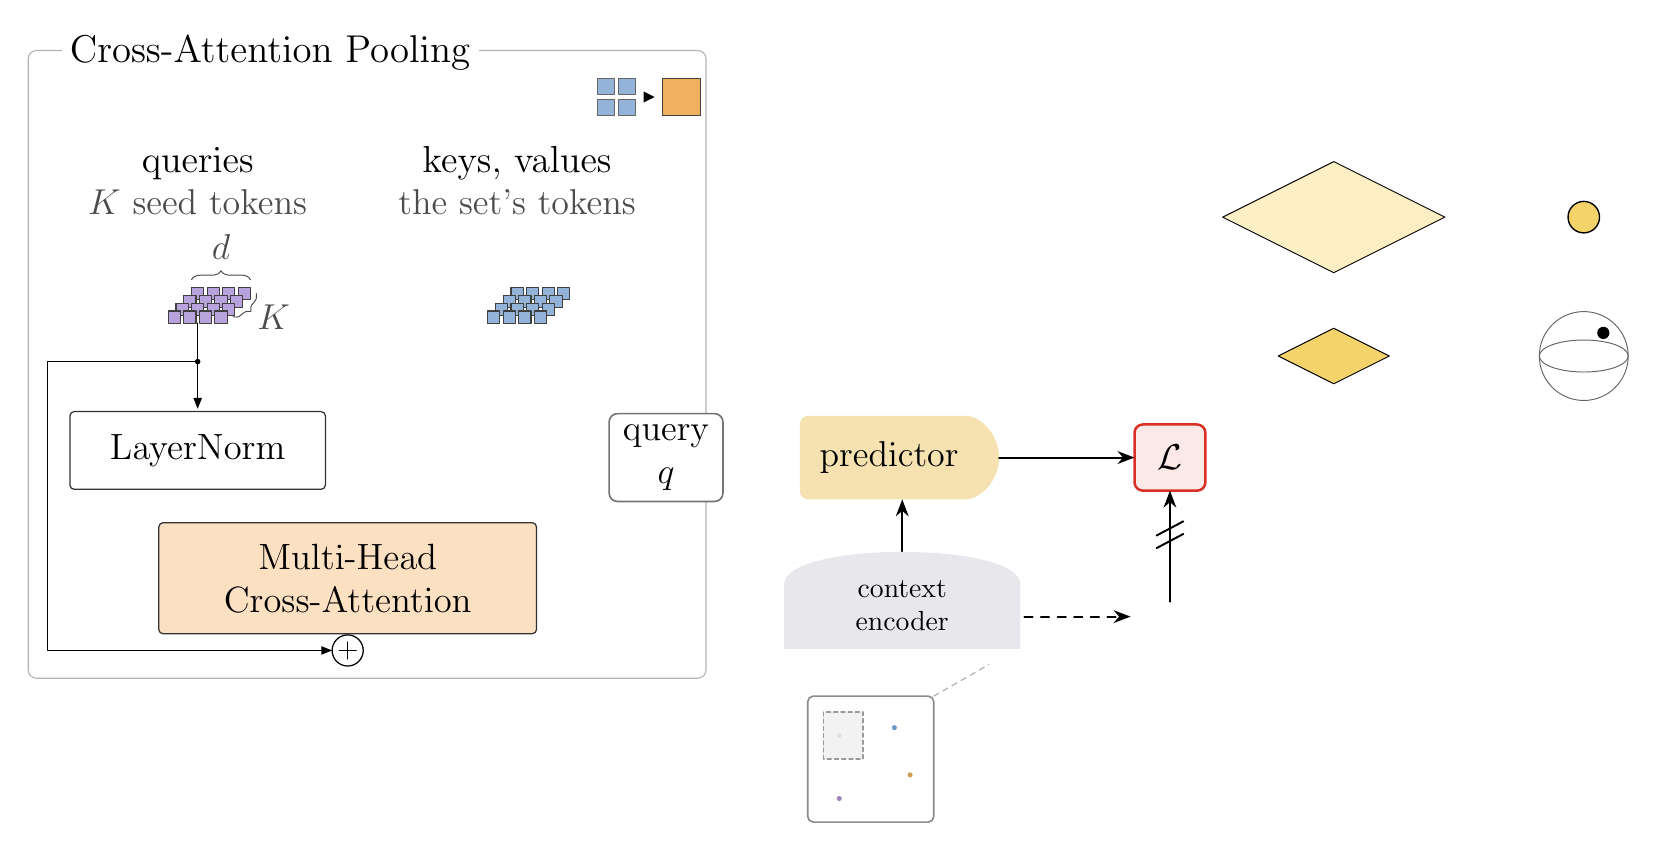
\begin{tikzpicture}[x=1bp, y=1bp, paper]
  % a card with its name on the border and a mini icon
  \card{0,0}{244}{226}{Cross-Attention Pooling}
  \minipool{205,-10}
  \twolevel{61,-44}{queries}{$K$ seed tokens}
  \twolevel{176,-44}{keys, values}{the set's tokens}
  \tokstack{61,-96}{tokpurple}
  \tokwidthbrace{61,-96}{$d$}
  \tokdepthbrace{61,-96}{$K$}
  \tokstack{176,-96}{tokblue}
  \node[box] (ln) at (61,-144) {LayerNorm};
  \draw[wire] (61,-98.2) -- (61,-129);
  \node[opbox] (att) at (115,-190) {Multi-Head\\Cross-Attention};
  \joincircle{115,-216}
  \coordinate (tap) at (61,-112); \coordinate (side) at (7,0); \coordinate (jn) at (115,-216);
  \residual{tap}{side}{jn}
  % overview family, in cm, beside the card
  \begin{scope}[x=1cm, y=1cm, shift={(9.6cm,-7.6cm)}]
    \slab{0,0}{3.0}{context\\encoder}
    \dcap{0.2,1.9}{2.0}{1.06}{predictor}
    \draw[flow] (1.5,1.24) -- (1.5,1.9);
    \node[qbox] at (-1.5,2.43) {query\\$q$};
    \node[loss] at (4.9,2.43) {$\mathcal{L}$};
    \draw[flow] (2.73,2.43) -- (4.45,2.43);
    \draw[ema] (3.05,0.41) -- (4.4,0.41);
    \draw[flowbare] (4.9,0.6) -- (4.9,1.2); \draw[flow] (4.9,1.2) -- (4.9,2.01);
    \stopgrad{4.9,1.45}
    \draw[crop] (0.3,-2.2) rectangle (1.9,-0.6);
    \draw[maskbox] (0.5,-1.4) rectangle (1.0,-0.8);
    \figpoint{1.4,-1.0}{ptblue} \figpoint{1.6,-1.6}{ptochre} \figpoint{0.7,-1.9}{ptpurple}
    \figmasked{0.7,-1.1}
    \draw[zoomlink] (1.9,-0.6) -- (2.6,-0.2);
  \end{scope}
  \isotile{470,-60}{40}{tilepale}
  \isotile{470,-110}{20}{tilestrong}
  \node[treenode, fill=tilestrong] at (560,-60) {};
  \unitsphere{560,-110}{16}
\end{tikzpicture}
\end{document}
